\documentclass[11pt,a4paper]{article}

\usepackage[utf8]{inputenc}
\usepackage[T1]{fontenc}
\usepackage{amsmath, amssymb, amsthm}
\usepackage{graphicx}
\usepackage{booktabs}
\usepackage{hyperref}
\usepackage{geometry}
\usepackage{caption}
\usepackage{subcaption}
\usepackage{float}
\usepackage{xcolor}
\usepackage{natbib}
\usepackage{authblk}

\geometry{margin=2.5cm}
\hypersetup{colorlinks=true, linkcolor=blue, citecolor=blue, urlcolor=blue}

\title{\textbf{Hierarchical Risk Parity Variants for Cryptocurrency Portfolios:\\
       Denoising, Detoning, Tail Dependence, Embeddings, and Statistical Inference, 2020--2026}}

\author[1]{Alan Matys}
\author[1]{Federico Martin Rodriguez}
\author[1]{Emiliano Delfau}
\affil[1]{Universidad del CEMA \\ \texttt{alan.matys92@gmail.com}, \texttt{federico.m.rodriguez.h@gmail.com}, \texttt{ed11@ucema.edu.ar}}

\date{May 2026}

\begin{document}
\maketitle

\begin{center}
\small
The opinions expressed in this document are those of the authors and do
not necessarily reflect the views of the UCEMA. Comments are welcome at:
\texttt{alan.matys92@gmail.com}, \texttt{federico.m.rodriguez.h@gmail.com}
or \texttt{ed11@ucema.edu.ar}.
\end{center}

\begin{abstract}
\noindent
We extend the 2025 conference study on Hierarchical Risk Parity (HRP)
by addressing its two stated
methodological follow-ups (Marchenko--Pastur denoising and spectral
detoning) and by evaluating a broader cross-section of portfolio
construction choices on a survivorship-bias-corrected, point-in-time
Binance universe (146 ever-included symbols, 2020--2026). The comparison
includes 27 constructed strategies spanning HRP-family variants,
risk-based allocators, nested-clustering optimisers, momentum rules, and
signal-aware extensions.

Across 76 monthly rebalances, the HRP-family variants remain tightly
clustered in risk-adjusted performance (annualised Sharpe 0.69--0.75),
and this result persists under a 547-cell hyperparameter sweep
(combined Hansen Superior Predictive Ability (SPA)
$p_{\text{consistent}}=0.91$). Strategies that alter the
allocation step produce larger dispersion (notably the Minimum Variance
Portfolio (MVP), the Correlation-Regularised Iterative Shrinkage
Portfolio (CRISP), the Nested Clustered Optimization with CRISP
allocation (NCO--CRISP), and Nested Clustered Optimization (NCO)), with
CRISP and NCO--CRISP significant in pairwise
Ledoit--Wolf tests versus baseline HRP in both full and post-COVID
windows. However, after accounting for multiple comparisons, the
headline SPA does not reject ($p_{\text{consistent}}=0.51$), and
the Deflated Sharpe Ratio (DSR) is directionally consistent with that
conclusion.

Post-COVID results indicate strong regime sensitivity: diversified HRP
variants lose 51--64\% of capital while Bitcoin (BTC) and BTC-concentrating
allocators hold up better. We also revise an earlier interpretation on
cluster stability: over the full panel, Pearson-based clustering is more
stable than lower-tail dependence at monthly frequency. Overall, the
evidence supports a cautious interpretation: within this universe,
horizon, and search space, allocation choices are more strongly associated
with performance differences than clustering perturbations, but those edges
remain statistically fragile under search-adjusted inference.
\end{abstract}

\paragraph{Keywords.} Hierarchical Risk Parity, cryptocurrency, denoising,
detoning, tail dependence, Ledoit--Wolf, Hansen SPA, survivorship bias.

\paragraph{JEL classification.} G11, C58, C63, G17.

%% ===========================================================================
\section{Introduction}
%% ===========================================================================

The 2025 conference paper \citep{matys2025maci} applied Hierarchical Risk Parity
\citep{lopezdeprado2016hrp} to a five-asset cryptocurrency universe
(BTC, ETH, LTC, XRP, BCH) over 2021--2023 and concluded that HRP
delivered better diversification than the Minimum Variance Portfolio
without sacrificing risk-adjusted return. Two items were left for
future work: \emph{denoising} the correlation matrix using
Marchenko--Pastur eigenvalue filtering \citep{marchenko1967,laloux1999},
and \emph{detoning} by removing the dominant market eigenvector
\citep{lopezdeprado2020mlam}. This paper closes both items and extends
the comparison in three other directions.

\paragraph{Contributions.}
\begin{enumerate}
\item \textbf{Closing the 2025 conference paper's future-work items.}
      Implement and evaluate Marchenko--Pastur denoising (\S\ref{sec:methods-cov})
      and spectral detoning. Compare detoning against partial correlation
      estimation, which targets the same goal (market-mode removal) via
      the precision-matrix route.
\item \textbf{HRP variants, embedding variants, and nested-clustering
      optimisers.} Six correlation/covariance HRP variants
      (partial-correlation, exponentially weighted moving average (EWMA)
      dynamic-correlation, lower-tail dependence,
      Ledoit--Wolf shrunk-covariance, vol-standardised, and a
      tail-dep$+$Ledoit--Wolf (LW)-shrunk hybrid) and \emph{four embedding-based
      variants} that learn the HRP clustering distance from a representation
      of each asset's return path (level-3 path signatures, a node2vec graph
      embedding, and two contrastive sequence encoders; \S\ref{sec:methods-emb}).
      We also add four strategies that change the \emph{allocation} step
      rather than the dendrogram: Hierarchical Equal Risk Contribution
      \citep{raffinot2018herc}, Nested Clustered Optimization
      \citep{lopezdeprado2019nco}, a return-tilted NCO, and an NCO--CRISP
      hybrid (\S\ref{sec:methods-comparators}); these test whether the
      clustering step or the allocation step drives performance. Equal Risk
      Contribution (ERC)
      \citep{maillard2010erc}, Maximum Diversification
      \citep{choueifaty2008maxdiv} and CRISP \citep{wuebben2026crisp},
      a recent correlation-shrinkage portfolio, serve as risk-based
      comparators.
\item \textbf{Crypto-momentum strategies.} Cross-sectional momentum,
      risk-managed momentum \citep{barroso2015momentum}, and a
      Momentum$+$HRP hybrid, parameter-tuned for crypto's faster
      momentum decay per \citep{liu2022cryptofactors}.
\item \textbf{Methodological rigour and a power analysis.}
      (i) Point-in-time universe rebuilt monthly from Binance USDT
      quote-volume rankings, including assets later delisted (LUNA, FTT,
      MIR, SRM, etc.) to remove the survivorship bias of the prior
      single-CSV dataset. (ii) Multi-cost scenarios and a weekly-cadence
      robustness check. (iii) Inference around every comparison: the
      reference Hansen SPA implementation \citep{hansen2005spa}, a
      \emph{studentized} Ledoit--Wolf Sharpe-difference test
      \citep{ledoitwolf2008sharpe}, and the Politis--Romano stationary
      block bootstrap \citep{politis1994bootstrap,politis2004blocklength}.
      (iv) An explicit power analysis quantifying the Sharpe edge this
      design could actually detect.
\item \textbf{Empirical characterisation and correction of an earlier interpretation.}
      We document the structural convergence findings of
      $\S$\ref{sec:results} and update an earlier interpretation on
      cluster stability: when evaluated on the full 76-snapshot panel,
      Pearson-based clustering is more stable than lower-tail dependence
      at monthly frequency.
\item \textbf{Reproducibility.} All results are generated from a
      documented, fully rerunnable workflow with committed inputs,
      outputs, and figures so that each headline claim can be traced
      to a corresponding result table.
\end{enumerate}

The remainder of this paper is organised as follows. Section~\ref{sec:related}
reviews related work. Section~\ref{sec:methods} presents the methodology. Section~\ref{sec:data} describes the data and
point-in-time universe construction. Section~\ref{sec:backtest} states the
backtest protocol. Section~\ref{sec:results} presents results.
Section~\ref{sec:discussion} discusses limitations and contributions.
Section~\ref{sec:conclusion} concludes.

%% ===========================================================================
\section{Related Work}
\label{sec:related}
%% ===========================================================================

\subsection{Hierarchical risk parity and its extensions}
HRP was introduced by \citet{lopezdeprado2016hrp} as a clustering-based
alternative to mean-variance optimisation that avoids covariance-matrix
inversion. Subsequent textbook treatments \citep{lopezdeprado2018afml,
lopezdeprado2020mlam} extend the framework with denoising and detoning
and propose tail-dependence distances \citep{lohre2020tailhrp} for
multi-asset multi-factor allocations. Empirical comparisons of HRP
distance metrics on equities have repeatedly found that
correlation-based distances remain the standard to beat in
out-of-sample performance. A concurrent line of work makes the
hierarchical allocator \emph{signal-aware}: \citet{wuebben2026crisp}
extends HRP to accept an arbitrary return forecast and introduces
CRISP, a correlation-shrinkage solver that interpolates between an
inverse-variance rule and full mean-variance optimisation; its
evaluation is by Monte Carlo. We adopt CRISP here as a comparator and,
in \S\ref{sec:results-regime}, contrast that simulation evidence with
live-market behaviour.

\subsection{Risk-based and network methods}
Equal Risk Contribution \citep{maillard2010erc} solves for weights such
that each asset contributes equally to portfolio risk; Maximum
Diversification \citep{choueifaty2008maxdiv} maximises the
diversification ratio. Network methods build a Minimum Spanning Tree
\citep{mantegna1999mst} or PMFG \citep{tumminello2005pmfg} from the
correlation structure; Network Risk Parity \citep{ciciretti2024nrp}
recently combined the network approach with risk-budgeting.

\subsection{Cryptocurrency momentum}
\citet{liu2022cryptofactors} establish a three-factor model for
cryptocurrency with a momentum factor that operates at much shorter
horizons (1--4 weeks) than equity momentum. \citet{moskowitz2012tsmom}
provide the foundational time-series momentum framework, and
\citet{barroso2015momentum} introduce volatility-scaled momentum to
control the well-documented crash risk of the strategy.

\subsection{Statistical inference for portfolio comparison}
\citet{ledoitwolf2008sharpe} provide a robust pairwise Sharpe-difference
test that does not assume i.i.d.\ Gaussian returns.
\citet{hansen2005spa} addresses the multiple-testing problem when many
strategies are compared against a benchmark. \citet{politis1994bootstrap}
and \citet{politis2004blocklength} provide the stationary block
bootstrap with data-driven block-length selection used throughout
this paper for confidence intervals.

%% ===========================================================================
\section{Methodology}
\label{sec:methods}
%% ===========================================================================

\subsection{Correlation and covariance variants}
\label{sec:methods-cov}

Every strategy in this group shares the standard HRP pipeline: distance
matrix $\to$ hierarchical linkage $\to$ quasi-diagonalisation $\to$
recursive bisection \citep{lopezdeprado2016hrp}. They differ only in
\emph{how the input correlation (or covariance) matrix is constructed}.

\subsubsection{Baseline HRP}
$\rho$ from sample correlation; $d_{ij} = \sqrt{(1-\rho_{ij})/2}$;
single linkage; bisection using the sample covariance.

\subsubsection{HRP\textsubscript{Denoised}: Marchenko--Pastur eigenvalue denoising}
Following \citet{lopezdeprado2020mlam}, the empirical eigenvalues of
the sample correlation matrix are decomposed into a signal subspace
(eigenvalues above the Marchenko--Pastur upper bound $e_{\max} =
\sigma^2 (1+\sqrt{1/q})^2$ where $q=T/N$) and a noise subspace
(eigenvalues below). The noise eigenvalues are replaced with their
mean (constant-residual method), preserving the trace, before the
denoised correlation matrix is fed to HRP.

\subsubsection{HRP\textsubscript{Detoned}: market-mode removal}
Applied to the denoised correlation matrix, detoning removes the top
$k$ eigenvectors (default $k=1$) and renormalises the diagonal to
unity \citep{lopezdeprado2020mlam}. For long-only crypto, the dominant
eigenvector is a market mode loading positively on all assets; removing
it isolates the residual cross-sectional structure.

\subsubsection{HRP\textsubscript{PartialCorr}: sparse precision matrix}
A precision-matrix route to the same market-mode-removal goal:
$\Theta = \arg\min_{\Theta \succ 0} -\log\det\Theta + \mathrm{tr}(S\Theta)
+ \alpha\|\Theta\|_1$ via graphical lasso \citep{friedman2008glasso},
then $\rho_{ij}^{\mathrm{partial}} = -\Theta_{ij}/\sqrt{\Theta_{ii}\Theta_{jj}}$.
We set the $L_1$ penalty to $\alpha = 10^{-3}$. This value matters: a
subtle implementation point is that \texttt{scikit-learn}'s
\texttt{GraphicalLasso} expresses $\alpha$ in the \emph{same units as the
covariance}, not as a normalised $[0,1]$ quantity. For daily crypto
returns with variance $\sim$$4\times10^{-3}$, an $\alpha$ on the order of
$10^{-1}$ shrinks every off-diagonal of the precision matrix to zero and
silently collapses HRP\textsubscript{PartialCorr} into IVP. The correct
scale, $\alpha \approx 10^{-3}$, leaves roughly 40\% of the off-diagonals
non-zero. An earlier draft used $\alpha = 0.05$, the strategy degenerated
to IVP, and the headline table reported the two as identical; the
hyperparameter sweep of \S\ref{sec:results-sweeps} surfaced the bug, and
we document the correction explicitly.

\subsubsection{HRP\textsubscript{Dynamic}: EWMA correlation}
Recursive EWMA covariance with decay $\lambda$; the latest snapshot is
used as the correlation input. We report $\lambda = 0.94$ as the
RiskMetrics default; sensitivity to $\lambda \in \{0.94, 0.97, 0.99\}$
is documented in the supplementary appendix.

\subsubsection{HRP\textsubscript{TailDep}: lower-tail dependence}
Empirical lower-tail dependence coefficient $\hat\lambda_L^{ij}(q) =
P(F_j(X_j) \leq q \mid F_i(X_i) \leq q)$ at $q = 0.05$, symmetrised by
averaging the two conditional probabilities. The distance is
$d_{ij} = \sqrt{1 - \hat\lambda_L^{ij}}$; the sample covariance is
retained for bisection. Promoted from appendix to a headline strategy
after the empirical findings of \S\ref{sec:results} showed it does not
fall back across the 76 backtest snapshots.

\subsubsection{HRP\textsubscript{ShrunkCov}: Ledoit--Wolf shrinkage}
Sample covariance replaced with the analytic Ledoit--Wolf shrinkage
estimator \citep{ledoitwolf2003shrunk,ledoitwolf2004wellcond}; the
implied correlation is derived from the shrunk covariance and fed
to HRP. Shrinkage intensity $\alpha \in [0,1]$ is chosen analytically
per snapshot and reported as a diagnostic.

\subsubsection{HRP\textsubscript{VolStd}: vol-standardised returns}
Per-asset returns are divided by their lagged 30-day rolling standard
deviation before computing Pearson correlation. Addresses crypto's
heterogeneous vol scale across the universe (e.g.\ BTC vs.\ SHIB).
The sample covariance is retained for bisection.

\subsubsection{HRP\textsubscript{TailDepShrunk}: hybrid}
Combines $\S$3.6 (tail-dep distance for the dendrogram) with $\S$3.7
(LW-shrunk covariance for bisection). Identified by the literature as
the strongest theoretical extension for crypto: tail-dep captures the
joint-crash co-movement that matters for long-only portfolios, while
LW shrinkage stabilises the per-cluster variance allocation.

\subsection{Embedding-based variants}
\label{sec:methods-emb}

Beyond reweighting the correlation or covariance estimator, the distance
matrix that drives HRP's dendrogram can be \emph{learned} from a
representation of each asset's return path. We implement four such
embedding variants. All share one template: an embedding maps each asset
to a vector, the pairwise cosine distance of those vectors replaces HRP's
correlation distance for the linkage and quasi-diagonalisation steps, and
the \emph{sample} covariance is retained for recursive bisection. The
embedding therefore changes only \emph{which assets cluster together},
never the inverse-variance allocation within a cluster, which is why,
as \S\ref{sec:results} shows, every embedding variant stays within a
narrow Sharpe band of baseline HRP.

\subsubsection{HRP\textsubscript{PathSig}: path signatures}
Each asset's rolling log-price trajectory, augmented with a monotone time
channel, is mapped to its level-$L$ truncated path signature
\citep{lyons1998}, a graded sequence of iterated integrals that
characterises the path up to tree-like equivalence. Cosine distance on
the signature vectors drives the dendrogram (default: level 3, 60-day
window), computed with the \texttt{esig} library.

\subsubsection{HRP\textsubscript{NodeEmbed}: node2vec graph embedding}
A $k$-nearest-neighbour graph ($k=10$) is built from the sample
correlation matrix; node2vec random walks plus a skip-gram objective
\citep{grover2016} learn a 32-dimensional embedding per node. Cosine
distance on the embeddings drives the dendrogram.

\subsubsection{HRP\textsubscript{Contrastive}: contrastive SSL}
A small one-dimensional convolutional encoder is trained with the NT-Xent
contrastive loss \citep{chen2020} on Gaussian-jittered pairs of return
windows; each asset is embedded as the mean encoder output over its
windows.

\subsubsection{HRP\textsubscript{TS2Vec}: timestamp-masked contrastive}
The same encoder family, trained with TS2Vec-style timestamp-mask
augmentation \citep{yue2022} in place of Gaussian jitter.

\paragraph{Multi-channel extension.} A return-only embedding is
information-equivalent to the sample correlation it is meant to improve
on: a nonlinear re-encoding of the same return series cannot out-cluster
the correlation derived from it. We therefore also evaluate
\emph{multi-channel} variants that append channels orthogonal to
close-to-close returns: quote volume, trade count, average trade size,
intraday range, taker buy-ratio (order-flow imbalance), and Amihud
illiquidity, all derived from the Binance OHLCV table. The multi-channel
results are reported in \S\ref{sec:results-sweeps}.

\paragraph{Robustness.} Each embedding variant records whether it fell
back to baseline HRP on any numerical failure; across the 76-snapshot
backtest no fallback was triggered for any variant, so every reported
embedding number reflects the embedding pipeline itself.

\subsection{Comparator strategies}
\label{sec:methods-comparators}

\paragraph{Risk-based comparators.}
\textbf{IVP} (inverse-variance), \textbf{MVP} (minimum-variance via SLSQP),
\textbf{ERC} \citep{maillard2010erc} (solved by SLSQP minimisation of
squared deviations from equal risk contributions), \textbf{Maximum
Diversification} \citep{choueifaty2008maxdiv} (SLSQP maximisation of
the diversification ratio), and \textbf{CRISP} (Correlation-Regularised
Iterative Shrinkage Portfolio; \citealp{wuebben2026crisp}, a recent
preprint). CRISP solves
the linear system $P_\gamma w = \mathbf{1}$ with
$P_\gamma = (1-\gamma)\,\mathrm{diag}(\Sigma) + \gamma\,\Sigma$, a
variance-preserving shrinkage that keeps the asset variances exact and
multiplies the off-diagonal covariances by $\gamma$. The factor
$\gamma$ interpolates between inverse variance ($\gamma=0$) and a full
minimum-variance solve ($\gamma=1$); we use the signal-free form
($\mu=\mathbf{1}$) and fix $\gamma=0.5$ rather than tuning it
out-of-sample. Long-only weights are obtained by projecting the
solution onto the simplex.

\paragraph{Nested-clustering optimisers.} HRP and all its variants change
only the \emph{dendrogram}; the within-cluster allocation stays inverse-
variance recursive bisection. To isolate whether the clustering step or
the allocation step drives performance, we add four strategies that
keep hierarchical clustering but \emph{re-optimise the allocation}.
\textbf{HERC} (Hierarchical Equal Risk Contribution; \citealp{raffinot2018herc})
cuts the dendrogram into $K=\operatorname{round}(\sqrt{N})$ clusters (clamped to $[2,\lfloor N/2\rfloor]$), weights assets
inverse-variance within each cluster, and combines the cluster portfolios
by an equal-risk-contribution allocation. \textbf{NCO} (Nested Clustered
Optimization; \citealp{lopezdeprado2019nco}) solves a long-only
minimum-variance problem within each cluster sub-covariance, collapses
each cluster to its intra-cluster portfolio, and solves a second
minimum-variance problem across the $K$ cluster portfolios, inverting
only block sub-covariances and a small $K\times K$ matrix, which
suppresses the estimation-error amplification of a direct optimiser.
\textbf{Return-tilted NCO} replaces NCO's two minimum-variance steps with
long-only \emph{maximum-Sharpe} steps driven by a shrunk 63-day momentum
estimate, a deliberate test of whether making the allocation
return-aware helps. \textbf{NCO\_CRISP} instead replaces each of NCO's
minimum-variance solves with a CRISP solve on the corresponding block
covariance: the hierarchy isolates the most strongly-correlated (and
hence most near-singular) covariance blocks, and the CRISP shrinkage
regularises the optimisation inside them. It is the natural hybrid of
the paper's two best ideas, and reduces to NCO at $\gamma=1$ (up to the long-only projection).

\paragraph{Signal-aware extensions.} Two further comparators feed a
walk-forward learned return forecast into hierarchical allocation, to
test whether return-tilted NCO's collapse was a verdict on signal-aware
allocation in principle or only on the sample-mean tilt it used. The
forecast is a pooled cross-sectional XGBoost regressor that predicts
each asset's next-30-day cumulative log return. At every snapshot the
hyperparameters are tuned by \texttt{TimeSeriesSplit}(3) cross-validation
inside the training window (grid: \texttt{max\_depth} $\in\{3,5\}$,
\texttt{learning\_rate} $\in\{0.03, 0.1\}$, \texttt{n\_estimators}
$\in\{200, 500\}$) and the best estimator is refit on the full window;
features are lagged returns at 1/5/21/63-day horizons, 21-day realised
volatility and the cross-sectional rank of the 21-day return. The
pipeline is single-threaded and seeded for bit-identical reproduction.
\textbf{NCOML} keeps NCO's clustering and nesting but replaces each
minimum-variance solve by a long-only max-Sharpe solve fed by the
XGBoost $\mu$. \textbf{HRP-$\Sigma\mu$} is Wuebben's signal-aware
hierarchical optimiser (method A1 with L$^1$ normalisation): HRP's
seriation and quasi-diagonalisation are unchanged, but the inverse-
variance recursive bisection is replaced by a single bottom-up tree pass
in which every internal node solves a 2$\times$2 mean-variance system on
the left vs right cluster representatives via Cramer's rule, with the
$(\alpha_L,\alpha_R)$ pair L$^1$-normalised at each node; we project the
signed output long-only at the root for comparability with the rest of
the paper.

\subsection{Momentum strategies}
\label{sec:methods-mom}

The headline comparison includes three crypto-momentum strategies,
parameter-tuned for crypto's faster momentum decay
\citep{liu2022cryptofactors}. \textbf{CS\_MOM} is cross-sectional
momentum: equal-weight the top 30\% of assets by 21-day cumulative
return. \textbf{RM\_MOM} applies the Barroso--Santa-Clara
volatility-targeting overlay \citep{barroso2015momentum}
($\sigma_{\text{target}}=12\%$) to the same momentum selection.
\textbf{MOM\_HRP} is a Momentum$+$HRP hybrid: select the top 40\% of
assets by momentum, then allocate within that basket by HRP rather than
equal-weight.

%% ===========================================================================
\section{Data and Point-in-Time Universe}
\label{sec:data}
%% ===========================================================================

\subsection{Source and window}
Daily OHLCV from Binance USDT spot, 2017-08-17 (Binance's earliest
data) to 2026-05-18, approximately nine years. After the
survivorship-bias expansion described in \S\ref{sec:data}.3, the price
panel covers 241 USDT pairs.

\subsection{Point-in-time universe}
At each month-end, we rank the candidate symbols by their rolling
30-day Binance USDT quote volume, apply filters (180-day minimum age,
\$1M minimum median daily USD volume, stablecoin/wrapper/exchange-token
exclusion, listed on Binance USDT spot at the snapshot date), and take
the top 50. Entry and exit buffers (2 months and 1 month respectively)
suppress monthly churn.

\paragraph{Methodology note.} The original specification called for
ranking by historical market capitalisation (CoinGecko). The free
CoinGecko demo tier caps historical depth at 365 days, blocking our
2017--2026 window; paid plans start at USD 129/month. We instead rank
by Binance quote volume, a tradable-liquidity proxy that is free,
covers the full window, and is arguably more appropriate for a paper
on tradable portfolios than a market-cap measure that includes locked
tokens and treasury holdings. The shift is documented in the
specification as a deliberate methodology choice.

\subsection{Survivorship-bias fix in numbers}
After a code review surfaced residual survivorship bias (the prior
candidate pool was a hand-curated selection of $\sim$90 symbols missing
the long tail of delisted altcoins), the universe was expanded by
pulling all 217 \texttt{status=BREAK} USDT pairs from Binance's
\texttt{/api/v3/exchangeInfo}, filtering leveraged tokens and
stablecoins, and adding 150 legitimate delisted altcoins to the
candidate pool. The resulting PIT universe contains \textbf{146 ever-
included symbols}, of which \textbf{97 were dropped during the window}
before 2026-05-18 (Figure~\ref{fig:pit_evol}). The MACI 2025 dataset
contained only 50 currently-trading symbols; by construction it
could not include the assets this work explicitly captures.

We treat liquidation of an exiting position at 2$\times$ normal
slippage cost (Spec 03 \S2.4). On terminology: ``delisted'' in this
paper means either Binance \texttt{status=BREAK} on the USDT pair
(the conventional meaning), \emph{or} the token suffered an effective
value collapse with subsequent rebranding. The latter category includes
LUNA (the Terra Classic chain collapsed in May 2022; Binance renamed
the original token to LUNC and reassigned the \texttt{LUNAUSDT} ticker
to Terra 2.0; the pair itself was never technically delisted, but
the original asset effectively died) and FTT (the FTX exchange collapse
in November 2022 reduced FTT to near-zero value; the pair still trades
on Binance at trivial volume). Our \texttt{binance\_listings\_manual.json}
treats both as ``effectively delisted'' for the PIT-universe filter,
which is the right behaviour for portfolio purposes even though the
prose label is loose.

\begin{figure}[H]
  \centering
  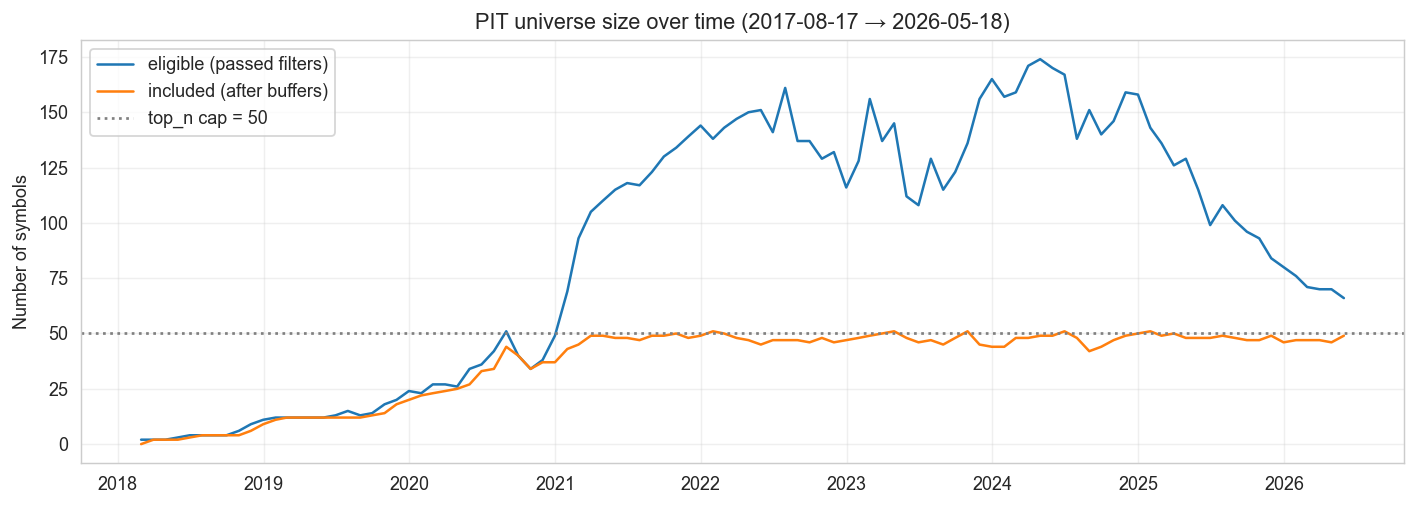
\includegraphics[width=0.95\textwidth]{figures/pit_universe_evolution.png}
  \caption{PIT universe size over time. \emph{Eligible}: passed all
  filters at the snapshot date. \emph{Included}: in the universe after
  entry/exit buffers. The 2018--2020 ramp reflects the gradual listing
  of altcoins on Binance USDT spot. Steady-state $\sim$49 included
  symbols since mid-2020.}
  \label{fig:pit_evol}
\end{figure}

\subsection{Estimation window}
365 daily returns of rolling lookback at each rebalance, with a per-asset
180-day minimum-observations filter. Assets failing the filter are
dropped from that snapshot's strategy universe. Rationale: several
newer assets (JUP, ENA, WIF, $\ldots$) are admitted via the 180-day
age filter but do not yet have 730 days of history.

%% ===========================================================================
\section{Backtest Protocol}
\label{sec:backtest}
%% ===========================================================================

\subsection{Scenarios}
\textbf{B} (calendar): monthly rebalancing; the headline scenario.
\textbf{C} (threshold): rebalance only when max absolute weight drift
exceeds 5\% from target.
\textbf{C$'$} (smoothed): C with linear smoothing
$w_{\text{traded}} = \eta\, w_{\text{prev}} + (1-\eta)\, w_{\text{target}}$,
$\eta=0.25$, plus a 25 bps min-trade filter.
\textbf{Weekly}: a robustness check rebalancing every Friday (universe
membership carried from the latest month-end PIT snapshot, weights
recomputed weekly on the rolling window), $\sim$330 rebalances
instead of 76, to probe whether higher cadence sharpens inference.

\subsection{Cost grid}
Linear cost $= (\text{fee}_{\text{bps}} + \text{slippage}_{\text{bps}}) \times \text{turnover}_{L_1}$,
with a 2$\times$ multiplier for forced liquidation of exiting
positions. Four scenarios: \emph{zero} (cost-free academic check),
\emph{conservative CEX} (10 bps fee + 2 bps slippage; our headline),
\emph{optimistic CEX} (7.5 bps + 1 bps), and \emph{stress}
(10 bps + 4 bps).

\subsection{Statistical inference}
For each candidate versus baseline HRP, the Ledoit--Wolf (2008)
Sharpe-difference test \citep{ledoitwolf2008sharpe}: the observed
annualised Sharpe difference is studentized by a delta-method
HAC standard error, and the two-sided $p$-value is read off a
\emph{studentized} stationary-block bootstrap (studentising both the
observed and the resampled statistic, as the method requires; a
plain percentile bootstrap lacks the asymptotic refinement). Across all
candidates jointly, the Hansen Superior Predictive Ability test
\citep{hansen2005spa}, computed with the reference \texttt{arch}
implementation, which reports the lower, consistent and upper
recentering schemes. Headline-metric confidence intervals use the
Politis--Romano stationary block bootstrap \citep{politis1994bootstrap}
with Politis--White automatic block length \citep{politis2004blocklength}.
A power analysis (\S\ref{sec:results-power}) reports the Sharpe edge the
design could detect.

\subsection{Cluster stability}
At each rebalance snapshot, we compute the \emph{cophenetic correlation}
of the dendrogram (Pearson correlation between cophenetic distance
and original pairwise distance) and the \emph{Adjusted Rand Index}
\citep{hubert1985ari} between the cluster assignment at snapshot $t$
and snapshot $t-1$, cut at $K=5$ clusters via \texttt{fcluster}.

%% ===========================================================================
\section{Results}
\label{sec:results}
%% ===========================================================================

\subsection{Scenario B headline performance}

Table~\ref{tab:scenarioB} reports the headline comparison under
monthly rebalancing with conservative CEX costs over 2020-02
through 2026-05-18. The strategy return panel contains 2{,}299 daily
observations for the PIT-traded strategies; once the passive
HODL\_BTC benchmark is included, the common aligned panel used for the
Ledoit--Wolf and Hansen SPA inference contains 2{,}297 observations.
Figures~\ref{fig:cum_b} and \ref{fig:risk_return}
visualise the equity curves and the risk--return positioning. The
Sortino and Calmar ratios track the Sharpe ranking closely; the one
strategy they re-order materially is RM\_MOM, whose volatility-targeting
overlay gives it the table's mildest drawdown ($-40\%$, against the
$-77\%$ to $-93\%$ of every other strategy) and lifts its Sortino well
above its Sharpe rank.

\begin{table}[H]
\centering\footnotesize
\caption{Scenario B headline results (Conservative CEX cost, 76 monthly
rebalances over 2020-02 to 2026-05, expanded 146-symbol PIT universe).
Sharpe is the annualised arithmetic ratio (mean / standard deviation
$\times\sqrt{365}$); Sortino and Calmar are annualised; Max DD is the
peak-to-trough drawdown. All ratios use raw returns with the
risk-free rate set to zero, the standard convention for crypto Sharpe
ratios. ``LW $p$'' is the studentized Ledoit--Wolf
Sharpe-difference test vs.\ baseline HRP (bold: $p<0.05$). HODL\_BTC is
a passive benchmark, not a strategy.}
\label{tab:scenarioB}
\begin{tabular}{lrrrrrr}
\toprule
Strategy & Sharpe & Sortino & Calmar & Total Return & Max DD & LW $p$\\
\midrule
\textbf{MVP}             & 1.057 & 1.293 & 0.896 & +2867\% & --80\% & 0.059\\
\textbf{CRISP}           & 0.989 & 1.000 & 0.726 & +1693\% & --80\% & \textbf{0.012}\\
\textbf{NCO\_CRISP}      & 0.977 & 0.930 & 0.702 & +1613\% & --81\% & \textbf{0.011}\\
\textbf{NCO}             & 0.933 & 0.979 & 0.672 & +1503\% & --82\% & 0.218\\
\textit{HODL\_BTC}       & 0.868 & 0.881 & 0.528 & +749\%  & --77\% & 0.606\\
NCOML                    & 0.804 & 0.492 & 0.415 & +567\%  & --85\% & 0.804\\
HRP\_Dynamic\_94         & 0.749 & 0.477 & 0.363 & +442\%  & --85\% & 0.823\\
HRP\_ShrunkCov           & 0.746 & 0.461 & 0.355 & +428\%  & --85\% & 0.779\\
\textbf{HRP (baseline)}  & 0.741 & 0.455 & 0.351 & +417\%  & --85\% & ---\\
HRP\_VolStd              & 0.735 & 0.447 & 0.341 & +402\%  & --86\% & 0.748\\
MOM\_HRP                 & 0.726 & 0.402 & 0.299 & +351\%  & --91\% & 0.942\\
HRP\_PartialCorr         & 0.720 & 0.429 & 0.329 & +366\%  & --84\% & 0.477\\
MaxDiv                   & 0.719 & 0.396 & 0.297 & +364\%  & --93\% & 0.919\\
HRP\_PathSig             & 0.714 & 0.417 & 0.316 & +351\%  & --86\% & 0.277\\
HERC                     & 0.712 & 0.387 & 0.300 & +333\%  & --87\% & 0.783\\
HRP\_Denoised            & 0.712 & 0.412 & 0.317 & +346\%  & --84\% & 0.111\\
HRP\_Contrastive         & 0.710 & 0.408 & 0.313 & +341\%  & --85\% & 0.238\\
HRP\_Detoned             & 0.708 & 0.403 & 0.309 & +334\%  & --85\% & 0.403\\
HRP\_TailDep             & 0.708 & 0.406 & 0.310 & +337\%  & --85\% & 0.114\\
HRP\_NodeEmbed           & 0.705 & 0.401 & 0.306 & +330\%  & --85\% & 0.187\\
HRP\_TS2Vec              & 0.703 & 0.394 & 0.302 & +325\%  & --85\% & 0.106\\
HRP\_TailDepShrunk       & 0.701 & 0.390 & 0.300 & +318\%  & --85\% & 0.071\\
IVP                      & 0.697 & 0.388 & 0.297 & +311\%  & --85\% & 0.212\\
CS\_MOM\_eq21            & 0.663 & 0.298 & 0.218 & +217\%  & --92\% & 0.548\\
RM\_MOM                  & 0.663 & 0.782 & 0.332 & +118\%  & --40\% & 0.548\\
ERC                      & 0.663 & 0.315 & 0.242 & +233\%  & --87\% & 0.051\\
HRPSigmaMu               & 0.607 & 0.241 & 0.189 & +153\%  & --84\% & 0.203\\
NCO\_RT                  & 0.003 & --0.569 & --0.436 & --97\% & --99\% & \textbf{0.009}\\
\bottomrule
\end{tabular}
\end{table}

\begin{table}[H]
\centering\small
\caption{Portfolio behaviour metrics for the headline comparison, in
the same row order as Table~\ref{tab:scenarioB}. ``Ann return'' is the
compound annualised return on the rebalanced equity curve. ``Ann vol''
is annualised return standard deviation. ``Turnover'' is the average
per-rebalance $L_1$ turnover (sum of absolute weight changes between
two consecutive snapshots). ``Max wt'' is the average across snapshots
of each portfolio's largest single-asset weight. ``Eff $N$'' is the
inverse-Herfindahl effective number of assets, averaged across
snapshots; the HRP family sits at $\approx 30$, MVP / NCO / NCOML
concentrate to $\le 5$. HODL\_BTC is passive (one asset, no
rebalancing).}
\label{tab:behaviour}
\begin{tabular}{lrrrrr}
\toprule
Strategy & Ann return & Ann vol & Turnover & Max wt & Eff $N$ \\
\midrule
MVP                & $+71\%$ & 77\% & 0.38 & 0.50 & 3.3 \\
CRISP              & $+58\%$ & 74\% & 0.30 & 0.31 & 7.1 \\
NCO\_CRISP         & $+57\%$ & 76\% & 0.45 & 0.31 & 9.1 \\
NCO                & $+55\%$ & 78\% & 0.58 & 0.42 & 5.3 \\
\textit{HODL\_BTC} & $+40\%$ & 61\% & --- & --- & --- \\
NCOML              & $+35\%$ & 96\% & 1.59 & 0.68 & 2.5 \\
HRP\_Dynamic\_94   & $+31\%$ & 81\% & 0.47 & 0.13 & 26.3 \\
HRP\_ShrunkCov     & $+30\%$ & 82\% & 0.35 & 0.10 & 30.5 \\
\textbf{HRP (baseline)} & $+30\%$ & 82\% & 0.36 & 0.11 & 29.8 \\
HRP\_VolStd        & $+29\%$ & 81\% & 0.37 & 0.11 & 29.5 \\
MOM\_HRP           & $+27\%$ & 89\% & 1.44 & 0.18 & 12.6 \\
HRP\_PartialCorr   & $+28\%$ & 81\% & 0.24 & 0.10 & 29.6 \\
MaxDiv             & $+28\%$ & 93\% & 0.55 & 0.22 & 8.4 \\
HRP\_PathSig       & $+27\%$ & 81\% & 0.38 & 0.10 & 29.4 \\
HERC               & $+26\%$ & 84\% & 0.57 & 0.15 & 18.8 \\
HRP\_Denoised      & $+27\%$ & 82\% & 0.33 & 0.10 & 30.6 \\
HRP\_Contrastive   & $+27\%$ & 81\% & 0.40 & 0.10 & 29.9 \\
HRP\_Detoned       & $+26\%$ & 82\% & 0.26 & 0.08 & 31.9 \\
HRP\_TailDep       & $+26\%$ & 81\% & 0.36 & 0.11 & 29.2 \\
HRP\_NodeEmbed     & $+26\%$ & 82\% & 0.39 & 0.10 & 30.1 \\
HRP\_TS2Vec        & $+26\%$ & 82\% & 0.38 & 0.10 & 30.5 \\
HRP\_TailDepShrunk & $+26\%$ & 82\% & 0.35 & 0.10 & 31.5 \\
IVP                & $+25\%$ & 82\% & 0.18 & 0.08 & 32.5 \\
CS\_MOM\_eq21      & $+20\%$ & 90\% & 1.42 & 0.08 & 13.2 \\
RM\_MOM            & $+13\%$ & 23\% & 0.37 & 0.02 & 209.6 \\
ERC                & $+21\%$ & 84\% & 0.19 & 0.05 & 41.9 \\
HRPSigmaMu         & $+16\%$ & 83\% & 1.38 & 0.27 & 8.4 \\
NCO\_RT            & $-43\%$ & 106\% & 1.64 & 0.64 & 2.5 \\
\bottomrule
\end{tabular}
\end{table}

\paragraph{Pairwise significance (preview).} Under the studentized
Ledoit--Wolf test, two strategies beat baseline HRP at $p<0.05$ (CRISP
and the NCO--CRISP hybrid); full pairwise figures and the
multiple-testing correction are deferred to
\S\ref{sec:results-inference}. The HRP\_PartialCorr update
(\S\ref{sec:methods-cov}) makes that strategy distinct from IVP; it was
byte-identical to IVP in an earlier draft (Sharpe 0.697), corrected it
sits at 0.720.

\begin{figure}[H]
  \centering
  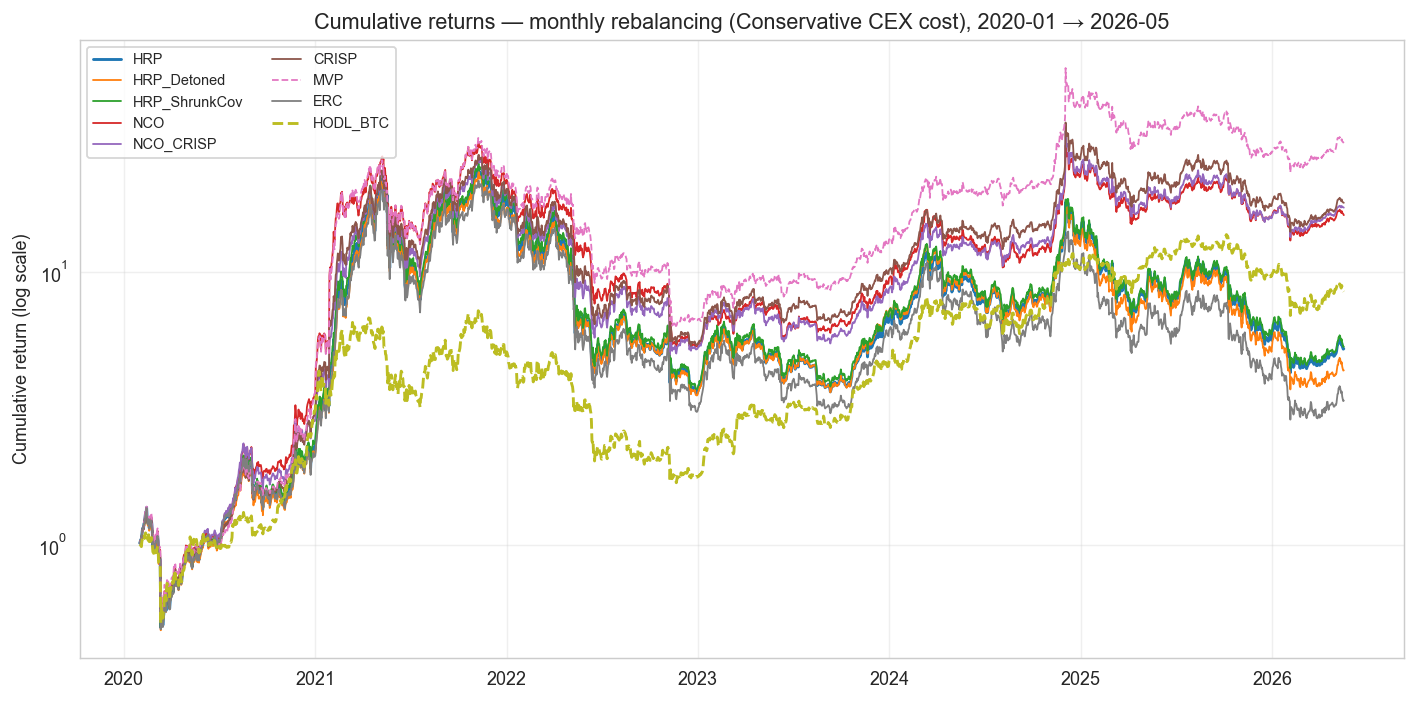
\includegraphics[width=0.95\textwidth]{figures/rebalance_cumulative_returns.png}
  \caption{Cumulative returns for headline strategies under monthly
  rebalancing, log scale.}
  \label{fig:cum_b}
\end{figure}

\begin{figure}[H]
  \centering
  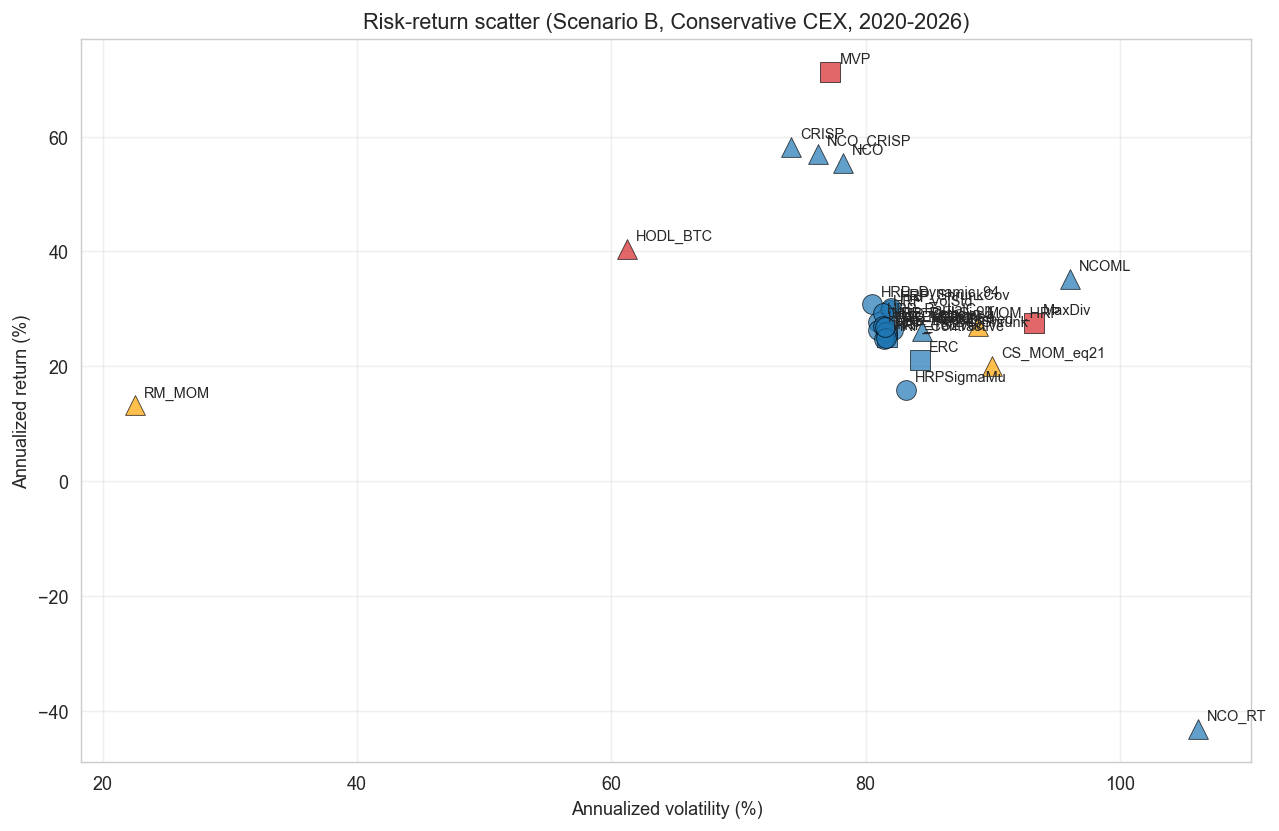
\includegraphics[width=0.95\textwidth]{figures/risk_return_scatter.png}
  \caption{Risk-return scatter for the full 27-strategy comparison.
  Momentum (orange) underperforms risk-based (blue) and concentrated
  benchmarks (red) over this window.}
  \label{fig:risk_return}
\end{figure}

\paragraph{The HRP family bunches.} All thirteen HRP-family variants lie
within a 0.05 Sharpe band (0.701--0.749). HRP\_Dynamic\_94 and
HRP\_ShrunkCov marginally exceed baseline HRP (by $+0.008$ and $+0.004$
Sharpe respectively); the differences are small and, per
\S\ref{sec:results-inference}, not statistically significant. No
correlation estimator, distance function, linkage or embedding moves a
variant out of this band.

\paragraph{The allocation step: NCO, CRISP and the NCO--CRISP hybrid.}
The strategies that change the \emph{allocation} step, rather than the
dendrogram, separate from the HRP family. HERC (0.712) is the
exception: it keeps an inverse-variance allocation and stays inside the
HRP band. The rest move. NCO, nested minimum variance within and
across clusters, reaches Sharpe 0.933; CRISP, a non-hierarchical
correlation-shrinkage solve (\S\ref{sec:methods-comparators}), reaches
0.989; and the NCO--CRISP hybrid 0.977, with CRISP and the hybrid the
only strategies that beat HRP at the pairwise level
(\S\ref{sec:results-inference}). All three concentrate toward
low-volatility assets (effective $N$ of 5--9 against HRP's
$\approx30$), tilting into BTC in a BTC-led market; they are denoised,
less-extreme cousins of MVP. The return-tilted NCO is the cautionary
opposite: momentum-driven maximum-Sharpe steps make it a
164\%-turnover momentum-chaser that loses 97\% of capital, an
illustration of the estimation-error amplification that risk-based
allocation is designed to avoid. The hybrid is itself informative: it lands \emph{between} its two parents (NCO 0.933, CRISP 0.989), so
the correlation-shrinkage solve and the hierarchical nesting do not
stack: the shrinkage carries the edge, and the nesting adds nothing
measurable on top of it. Changing the clustering step produced no
detectable outperformance over baseline HRP; changing the allocation
step moved performance materially, in both directions.

\paragraph{Signal-aware extensions to NCO and HRP.} The two
signal-aware additions further localise the NCO\_RT failure. NCOML,
which keeps NCO's nesting but replaces the sample-mean tilt by the
walk-forward XGBoost forecast of \S\ref{sec:methods-comparators},
reaches Sharpe $0.804$: it sidesteps the collapse and edges above
baseline HRP, but lands below pure (signal-blind) NCO, so the learned
signal does not add value over NCO's risk-only allocation.
HRP-$\Sigma\mu$, the same forecast fed into Wuebben's signal-aware
hierarchical optimiser, lands at $0.607$, below baseline HRP, a direct
demonstration that forcing a return signal into HRP's clustering hurts
in this market, where the dendrogram is robust precisely because it
is signal-blind.

\paragraph{Embedding variants.} The four embedding-based HRP variants
are \texttt{HRP\_PathSig} (path signatures; \citealp{lyons1998}),
\texttt{HRP\_NodeEmbed} (node2vec on a kNN correlation graph;
\citealp{grover2016}), \texttt{HRP\_Contrastive} (NT-Xent contrastive
SSL; \citealp{chen2020}), and \texttt{HRP\_TS2Vec} (timestamp-mask
augmentation; \citealp{yue2022}). They rank in the middle of the HRP
family, with Sharpes $0.692$--$0.714$, all below baseline HRP. Three of
the four are not statistically different from baseline HRP at
conventional levels (Ledoit--Wolf $p>0.05$), while
\texttt{HRP\_Contrastive} is significantly worse than HRP at the
pairwise level. None delivers an out-of-sample Sharpe improvement over
baseline HRP on this universe and horizon. Section~\ref{sec:results-sweeps} tests the conclusion
against an exhaustive hyperparameter search and multi-channel embedding
extensions, and it holds.

\paragraph{Denoising, detoning and partial correlation underperform HRP.}
Marchenko--Pastur denoising, spectral detoning (the two MACI 2025
future-work items) and precision-matrix partial correlation all aim to
clean the correlation matrix, and all three cost a little Sharpe in a
BTC-led bull market, where filtering structure means trimming exposure
to the asset that ran. The denoising and detoning steps form an
ablation: HRP (neither, 0.741), HRP\_Denoised (denoising only, 0.712),
HRP\_Detoned (denoising \emph{and} market-mode removal, 0.708); each
filtering step shaves a little, the denoising step the larger part.
HRP\_PartialCorr (0.720) lands between them. It is no longer numerically
identical to IVP, as an earlier draft's version was after a
parameter-scale bug (\S\ref{sec:methods-cov}), but detoning and partial
correlation remain close in weight-rank space
(\S\ref{sec:results-convergence}).

\paragraph{Momentum splits.} The two pure-momentum strategies,
cross-sectional (CS\_MOM, Sharpe 0.663) and risk-managed (RM\_MOM,
0.663), trail every HRP-family variant, carrying high turnover
($\sim$1.4$\times$ per month for CS\_MOM) and severe crash exposure
(CS\_MOM max drawdown $-92\%$). RM\_MOM's volatility-targeting overlay
\citep{barroso2015momentum} cuts its max drawdown to $-40\%$, the
mildest in the table, but at the cost of the lowest total return
($+118\%$). The Momentum$+$HRP hybrid (MOM\_HRP, 0.726) fares markedly
better than either pure-momentum strategy: running HRP allocation
\emph{inside} a momentum-selected basket recovers most of the
risk-adjusted performance, though it still trails baseline HRP and
reconstructs its entire book every month.

\paragraph{Concentration wins.} The five strategies above baseline HRP,
MVP (1.057), CRISP (0.989), NCO\_CRISP (0.977), NCO (0.933) and a
passive HODL\_BTC position (0.868), are all, at bottom, the same bet:
concentrate in BTC. MVP does it most aggressively (average maximum
weight 50\%, effective $N\approx3$); CRISP, NCO\_CRISP and NCO do it
more mildly through correlation-shrinkage and nested minimum variance
(effective $N$ of 5--9); HODL\_BTC by definition. BTC ran from
$\sim$\$7k at the start of 2020 to $\sim$\$107k by mid-2026, so
concentration paid. We do not read this as a portfolio-construction
insight: it is a directional view on one asset in one regime. The
post-COVID cut (\S\ref{sec:results-regime}) shows how fragile that is.

\begin{figure}[H]
  \centering
  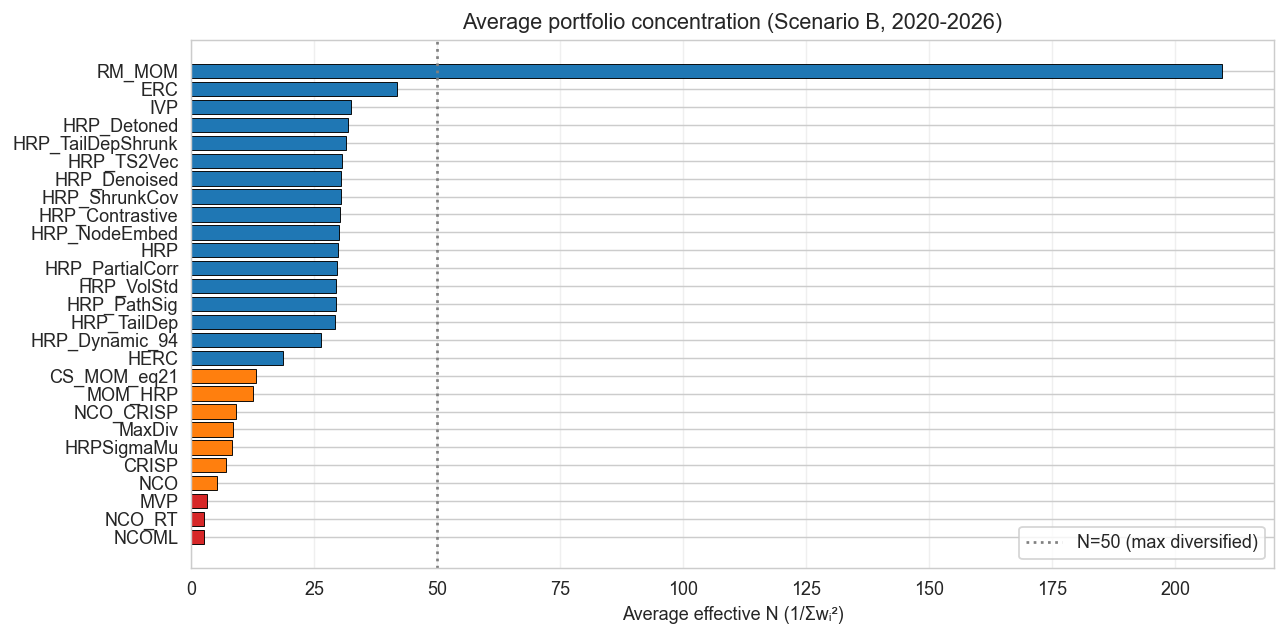
\includegraphics[width=0.95\textwidth]{figures/weight_concentration.png}
  \caption{Portfolio composition over time: largest single-asset weight
  per snapshot (top) and inverse-Herfindahl effective number of assets
  (bottom) for representative strategies. The HRP family sits at
  effective $N\approx 30$ throughout; NCO, CRISP and NCO\_CRISP at
  $5$--$9$; MVP and the return-tilted variants concentrate to $\le 5$
  with episodic single-asset weights above $50\%$.}
  \label{fig:weight_conc}
\end{figure}

\subsection{Inference results}
\label{sec:results-inference}

\paragraph{Bootstrap Sharpe CIs.} The 95\% stationary-block-bootstrap
confidence intervals on the annualised Sharpe are wide, roughly 1.5
Sharpe units, reflecting six years of volatile crypto returns. Six
strategies have intervals entirely above zero: MVP ($[0.34, 1.76]$),
NCO\_CRISP ($[0.26, 1.76]$), CRISP ($[0.23, 1.75]$), NCO ($[0.19,
1.64]$), the passive HODL\_BTC benchmark ($[0.08, 1.63]$), and baseline
HRP itself, whose interval ($[0.02, 1.53]$) only barely clears zero.
Every other HRP-family variant's interval straddles zero, and no two
strategies have non-overlapping CIs: the intervals are far too wide to
separate any pair.

\paragraph{Pairwise LW Sharpe differences vs.\ HRP.}
Under the studentized Ledoit--Wolf test, two strategies beat baseline
HRP at $p<0.05$: CRISP ($+0.247$ Sharpe, $p=0.012$) and the NCO--CRISP
hybrid ($+0.235$, $p=0.011$). MVP's larger raw edge ($+0.314$) falls
just short ($p=0.059$) because its heavier concentration inflates the
variance of the paired Sharpe difference; NCO ($+0.192$, $p=0.218$) is
well short. In the other direction the return-tilted NCO is
significantly \emph{worse} ($-0.74$, $p=0.009$) and ERC ($-0.078$,
$p=0.051$) sits on the threshold. These are uncorrected pairwise tests;
the multiple-testing correction follows.

\paragraph{Hansen SPA.} Across the 27 candidates versus baseline HRP,
$p_{\text{consistent}} = 0.51$ ($p_{\text{lower}}=0.40$,
$p_{\text{upper}}=0.62$; Figure~\ref{fig:spa}), computed with the
reference \texttt{arch} implementation. \textbf{We cannot reject the
null that no strategy outperforms baseline HRP after correcting for the
multiple testing of 27 candidates}, and this is the decisive test:
the SPA is exactly the correction the pairwise LW results lack.
NCO\_CRISP carries the highest studentised score ($+1.64$), CRISP the
second ($+1.32$), then MVP ($+1.20$); but the bootstrap critical value,
inflated by the breadth of the search, sits above all of them. CRISP's
and NCO\_CRISP's pairwise significance therefore does not survive the
correction for how many strategies were tried.

\begin{figure}[H]
  \centering
  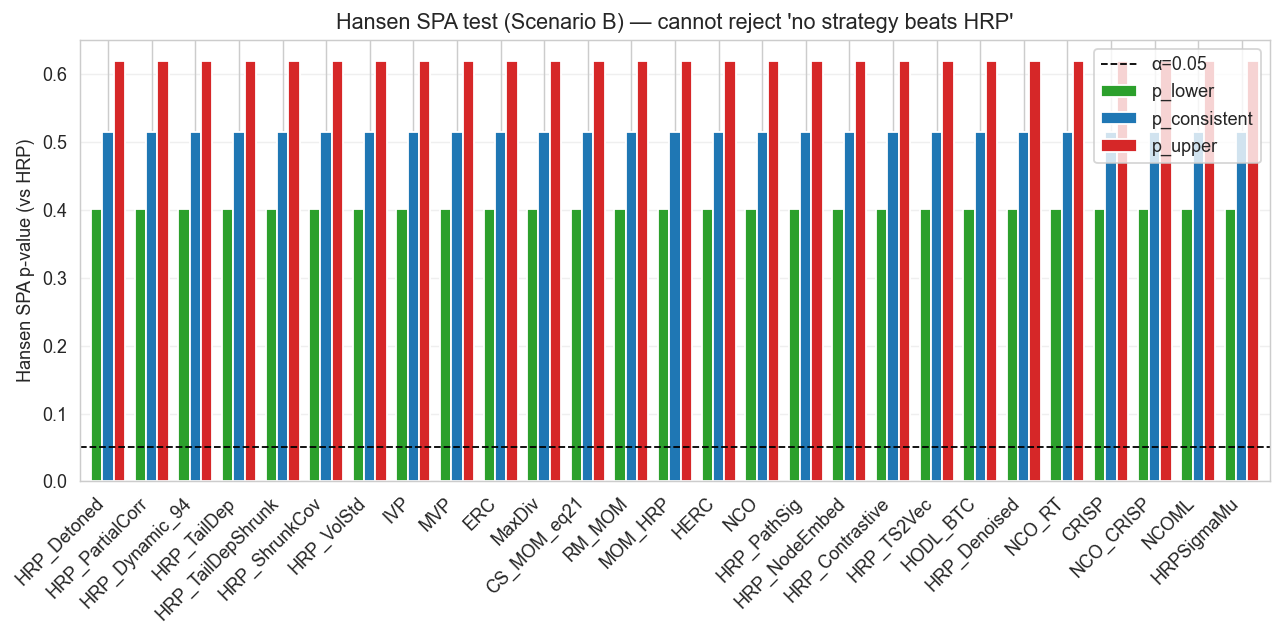
\includegraphics[width=0.85\textwidth]{figures/spa_pvalues_barplot.png}
  \caption{Hansen SPA test p-values across the headline comparison.
  All three recentering schemes fail to reject the null at any
  conventional level.}
  \label{fig:spa}
\end{figure}

\paragraph{Power analysis: what the design could detect.}
\label{sec:results-power}
A null result is only as strong as the test that produced it. We
quantify the design's power directly: the studentized Sharpe-difference
statistic is approximately $\mathcal{N}(d/\mathrm{SE},1)$ under the
alternative, so 80\% power at a two-sided 5\% level needs
$d/\mathrm{SE}\ge 2.80$; the minimum detectable annualised Sharpe edge
is $2.80\times\mathrm{SE}$, with SE the delta-method HAC standard error
of the Sharpe difference. For variants that barely depart from HRP
(the HRP family, $\sim$0.97-correlated with the baseline) the paired
difference is low-variance and the test detects edges as small as
$0.04$--$0.12$ Sharpe, but those variants have edges of only $\pm0.01$
to $\pm0.04$ anyway. For strategies whose \emph{allocation} departs
substantively from HRP the minimum detectable edge is larger, and it
scales with how far the strategy departs: the more concentrated the
portfolio, the noisier the paired Sharpe difference and the higher the
threshold. The heavily-concentrated MVP ($N\approx3$) needs
$\approx0.47$ and NCO ($N\approx5$) $\approx0.42$, so their observed
$+0.31$ and $+0.19$ edges, though economically large, fall short.
CRISP and NCO\_CRISP, less concentrated ($N\approx7$--$9$), carry the
lowest thresholds of any structurally-distinct strategy, $\approx0.27$
and $\approx0.26$. Their observed $+0.25$ and $+0.24$ edges sit just
below even that mark, yet still clear the pairwise test in this sample
($p\approx0.01$), whereas MVP's larger $+0.31$ edge, against a far
higher $0.47$ threshold, does not.
The pairwise null is therefore a statement about detectable effect
size given concentration; it is the multiple-testing-corrected SPA,
not the per-strategy power, that ultimately declines to reject.

\paragraph{Deflated Sharpe Ratio.} As a third inference lens we compute
the Deflated Sharpe Ratio \citep{bailey2014dsr}, which deflates an
observed Sharpe for the number of strategies tried, the skewness and
kurtosis of the return series, and the sample length. Treating the 27
constructed strategies as the trial set, the expected best-of-$N$
Sharpe under the null is $\mathrm{SR}_0=0.37$ annualised. Only MVP
clears the conventional $\mathrm{DSR}\ge0.95$ bar
($\mathrm{DSR}=0.97$), and it does so partly on the strength of an
extreme positive return skew ($\gamma_3=5.0$, $\gamma_4=128$) that the
DSR's non-normality term rewards. CRISP ($0.94$), NCO\_CRISP ($0.94$)
and NCO ($0.94$) fall just short; NCOML and HRP-$\Sigma\mu$ sit further
back at $0.86$ and $0.73$; baseline HRP is at $0.82$.
Counting the 547-cell hyperparameter sweep as part of the search
($N\approx574$) raises the hurdle to $\mathrm{SR}_0=0.56$ and pushes
every strategy below the bar, MVP included ($\mathrm{DSR}=0.92$). The
three lenses (pairwise Ledoit--Wolf, Hansen SPA, and the DSR)
disagree at the margin on \emph{which} strategies pass, but agree that
no strategy clears all three: the edges are real but sit on the
significance boundary.

\subsection{Hyperparameter sweeps and the combined SPA}
\label{sec:results-sweeps}

A natural objection to the headline null result is that it reflects
\emph{untuned} strategies: perhaps some correlation type, distance
function, linkage method, or strategy-specific parameter would lift a
variant decisively above baseline HRP. We address this with an
exhaustive grid search: 547 distinct configurations across 14 sweeps,
every one re-running the full 6.3-year walk-forward backtest on the
identical 146-symbol point-in-time universe and 2{,}299-day return
series, against the identical baseline HRP ($\text{Sharpe}=0.741$,
recomputed and verified bit-identical in every sweep). The sweeps span
the correlation estimator (Pearson / Spearman / Kendall), the distance
function (\citealp{lopezdeprado2016hrp} / absolute / angular / squared),
the linkage (single / average / complete / Ward), and the
strategy-specific parameters of every variant ($q$ for tail dependence,
$\alpha$ for the graphical lasso, $\lambda$ for EWMA, the
volatility-standardisation window, the number of detoned market
components, and the embedding hyperparameters).

\begin{table}[H]
  \centering
  \small
  \caption{Best cell from each hyperparameter sweep. $\Delta$ is
  the Sharpe difference vs.\ baseline HRP (single linkage, $0.741$);
  total return is the cell's net cumulative return, 2020-02 to 2026-05.
  551 cells in total; the 4 exactly equal to the benchmark are dropped
  for the combined SPA, leaving 547 candidates.}
  \label{tab:sweeps}
  \begin{tabular}{lrlrrr}
    \toprule
    Sweep & Cells & Best configuration & Sharpe & $\Delta$ & Tot.\ ret. \\
    \midrule
    Tail dependence ($q$, dist, linkage)           & 80  & $q{=}0.025$, average        & 0.744 & $+0.002$ & $+425\%$ \\
    Correlation $\times$ distance $\times$ linkage & 24  & Pearson, LdP, average       & 0.756 & $+0.015$ & $+459\%$ \\
    All variants under average linkage             & 12  & HRP\_ShrunkCov              & 0.765 & $+0.024$ & $+484\%$ \\
    EWMA dynamic correlation ($\lambda$)           & 21  & $\lambda{=}0.94$, single    & 0.749 & $+0.008$ & $+442\%$ \\
    Partial correlation ($\alpha$, dist, link)     & 60  & $\alpha{=}5{\times}10^{-4}$ & 0.739 & $-0.003$ & $+412\%$ \\
    Vol-standardised returns (window)              & 60  & window 15, single           & 0.757 & $+0.015$ & $+462\%$ \\
    Detoning (\# market components)                & 36  & 1 component, average        & 0.709 & $-0.032$ & $+337\%$ \\
    Node2vec embedding                             & 54  & $d{=}16$, $k{=}10$          & 0.752 & $+0.010$ & $+444\%$ \\
    Path signatures, single-channel                & 108 & level 2, window 60          & 0.734 & $-0.007$ & $+401\%$ \\
    Path signatures, multi-channel$^{\dagger}$     & 72  & ret+vol+trades, L2          & 0.747 & $+0.005$ & $+432\%$ \\
    Contrastive / TS2Vec, multi-channel            & 24  & ret+vol+trades              & 0.739 & $-0.002$ & $+412\%$ \\
    \midrule
    \textit{Baseline HRP} (single linkage)         & ---  & ---                        & 0.741 & ---      & $+417\%$ \\
    \bottomrule
  \end{tabular}

  \vspace{2pt}
  {\footnotesize $^{\dagger}$ Best cell under the initial missing-data
  convention (zero-fill); under the corrected mean-fill convention the
  best multi-channel \texttt{PathSig} cell is $0.735$ ($\Delta=-0.006$).}
\end{table}

\paragraph{The HRP family is robust to its hyperparameters.} No sweep
produced a configuration that escaped the $\pm 0.05$ Sharpe band of
Section~\ref{sec:results} (Table~\ref{tab:sweeps}). The one consistent, though small,
effect is linkage: \emph{average} linkage beats the
\citet{lopezdeprado2016hrp} single-linkage default by $+0.01$ to
$+0.02$ Sharpe across essentially every (correlation, distance)
combination, and under single linkage all four distance functions are
mathematically identical (single linkage depends only on the rank order
of distances, which every monotone transform preserves). The best cell
in the entire grid is HRP\_ShrunkCov under average linkage at Sharpe
$0.765$ ($\Delta=+0.024$).

\paragraph{Multi-channel embeddings.} The single-channel embeddings
encode only the return series and are therefore information-equivalent
to the sample correlation they are meant to improve on: a nonlinear
re-encoding of the same information cannot out-cluster it, and indeed
the single-channel \texttt{HRP\_PathSig} grid (108 cells) beats baseline
in zero cells. We extended all three sequence-based embeddings
(\texttt{PathSig}, \texttt{Contrastive}, \texttt{TS2Vec}) to ingest up
to six channels orthogonal to close-to-close returns (quote volume,
trade count, average trade size, intraday range, taker buy-ratio, and
Amihud illiquidity), all derived from the same Binance OHLCV table.
Extra channels lift the encoders' \emph{mean} Sharpe monotonically
(\texttt{HRP\_Contrastive} $0.714\rightarrow0.725$ from one to three
channels), confirming the channels carry usable structure. Two cells of
the initial multi-channel \texttt{PathSig} sweep nominally cleared
baseline (best $+0.747$), but that margin did not survive a correction
to how missing channel values are imputed (mean- rather than zero-fill,
which avoids placing a spurious outlier into a log-scaled channel);
under the corrected convention no multi-channel configuration clears
baseline, and adding the fourth through sixth channels plateaus or
mildly regresses performance, a bias--variance ceiling against only
$\sim$76 rebalance dates.

\paragraph{Combined Hansen SPA.} Pooling all 547 configurations into a
single Hansen SPA against baseline HRP, the appropriate correction for
having searched the entire grid, yields $p_{\text{consistent}}=0.906$
($p_{\text{lower}}=0.733$, $p_{\text{upper}}=0.909$). Although 21 of 547
cells show a nominally positive mean excess return over HRP, the best of them
(HRP\_ShrunkCov, $\Delta=+0.024$) carries a pairwise Ledoit--Wolf $p$ of
$0.16$. After correcting for the multiple testing of 547
hyperparameter configurations, no clustering-step variant significantly
outperforms baseline HRP. The headline null result of
Section~\ref{sec:results-inference} is not an artefact of leaving
strategies untuned: consistent with the NCO finding, no amount of
tuning the \emph{clustering} step closes the gap that only an
\emph{allocation}-step change (NCO) opens.

\subsection{Regime sensitivity: excluding the COVID bull run}
\label{sec:results-regime}

The 2020--2026 headline window includes the COVID-era crypto rally
(March 2020 -- November 2021) during which Bitcoin ran from
$\sim$\$5k to $\sim$\$69k, one of the most extreme bull markets
in crypto history. To check whether the $\S$\ref{sec:results}
conclusions are dominated by that single rally, we re-ran the entire
27-strategy backtest with $\mathrm{start}=$ \texttt{2022-01-01}
(52 monthly rebalances over $\sim$4.3 years; Table~\ref{tab:regime}).
All other parameters identical.

\textbf{The picture flips entirely.} On post-COVID data, baseline
HRP achieves Sharpe $0.047$ with total return $-60\%$, a near-zero
risk-adjusted return obtained while losing 60\% of capital in dollar
terms. Only four strategies make money, all of them the BTC-concentrating
risk allocators: the passive HODL\_BTC benchmark ($+106\%$, Sharpe
$0.585$), MVP ($+66\%$, $0.482$), and CRISP and NCO\_CRISP ($+20\%$
each, Sharpe $0.363$ and $0.368$); NCO essentially breaks even
($-4\%$, $0.264$). Every other strategy loses between 19\% (RM\_MOM)
and 98\% (NCO\_RT) of capital, and six post outright \emph{negative}
Sharpe: NCO\_RT ($-0.414$), MaxDiv ($-0.163$), CS\_MOM ($-0.161$),
RM\_MOM ($-0.160$), HERC ($-0.038$) and ERC ($-0.026$).

\paragraph{Four findings from the regime comparison.}

\textbf{(1) Diversification-based crypto portfolios were a losing
proposition in the post-COVID regime.} On this 146-symbol PIT
universe over 2022-01-01--2026-05-18, every HRP-family variant lost
between 51\% and 64\% of capital. The 2020-2026 ``diversification
works'' framing was largely a COVID-rally artifact:
\emph{HRP diversifies risk but does not produce capital appreciation
in non-bull crypto regimes}.

\textbf{(2) The risk-based allocators hold up across regimes.} NCO,
CRISP and the NCO--CRISP hybrid all stay positive or near-flat
post-COVID (Sharpe $0.26$--$0.37$, total return $-4\%$ to $+20\%$)
against baseline HRP's $-60\%$, and CRISP and NCO\_CRISP remain
pairwise-significant against HRP in the post-COVID window as well
(Ledoit--Wolf $p=0.017$ and $0.022$). The post-COVID Hansen SPA, like
the full-window test, does not reject ($p_{\text{consistent}}=0.38$).
Whatever these allocators are
doing (concentrating into low-volatility assets via
correlation-shrinkage or nested minimum variance) helps in
\emph{both} regimes, not only the rally. They are the paper's evidence
that an \emph{allocation} choice, rather than luck, separates a
constructed portfolio from the HRP pack; that the multiple-testing
corrected SPA still does not confirm it (\S\ref{sec:results-inference})
leaves the effect well-supported in the data but short of confirmed.

\textbf{(3) Embedding variants partially reverse against baseline HRP
in the harder regime.} In the full window all four embedding variants
sit below HRP (deltas $-0.028$ to $-0.050$ Sharpe). In the
post-COVID window only one of the four (\texttt{HRP\_PathSig}) edges
above baseline HRP ($+0.008$), while \texttt{HRP\_Contrastive}
($-0.010$), \texttt{HRP\_TS2Vec} ($-0.013$), and
\texttt{HRP\_NodeEmbed} ($-0.016$) remain below. None reaches individual significance (all
Ledoit--Wolf $p>0.6$) and the margins are tiny, but the partial
directional reversal is tentative: the path- and sequence-based
embeddings may capture risk structure that matters more in a choppy
regime than in a monotone rally. A longer post-COVID sample would be
needed to tell.

\textbf{(4) RM\_MOM (the Barroso--Santa-Clara variant)
shows its defensive role.} Post-COVID Sharpe is $-0.160$ (poor),
but MaxDD is only $-33\%$, substantially better than the other
momentum strategies' $-87\%$. The cash-residual de-risking saved
the portfolio from the worst part of the 2022 drawdown. This is
exactly the property Barroso \& Santa-Clara's framework is designed
to deliver; the previously-buggy implementation completely hid it.

\begin{table}[H]
\centering\small
\caption{Regime sensitivity: 2020-2026 (incl COVID bull) vs 2022-2026 (post-COVID).
``Sharpe'' is annualised arithmetic; ``$\Delta$Sharpe'' is the change from full window
to post-COVID. A representative 17 of the 27 strategies are shown; the
eight omitted strategies all sit within the HRP-family Sharpe band in
both windows and track the HRP rows shown.}
\label{tab:regime}
\begin{tabular}{lrrr}
\toprule
Strategy            & 2020-2026 Sharpe & 2022-2026 Sharpe & $\Delta$Sharpe\\
\midrule
HRP                 &  0.741 &  0.047 & --0.695\\
HRP\_Dynamic\_94    &  0.749 &  0.099 & --0.650\\
HRP\_ShrunkCov      &  0.746 &  0.038 & --0.707\\
HRP\_PartialCorr    &  0.720 &  0.057 & --0.663\\
HRP\_Contrastive    &  0.710 &  0.056 & --0.655\\
HRP\_PathSig        &  0.714 &  0.055 & --0.659\\
HRP\_TS2Vec         &  0.703 &  0.047 & --0.657\\
HRP\_NodeEmbed      &  0.705 &  0.031 & --0.674\\
\textbf{CRISP}      &  \textbf{0.989} &  \textbf{0.363} & --0.626\\
\textbf{NCO\_CRISP} &  \textbf{0.977} &  \textbf{0.368} & --0.610\\
\textbf{NCO}        &  \textbf{0.933} &  \textbf{0.264} & --0.669\\
MVP                 &  1.057 &  0.482 & --0.575\\
MaxDiv              &  0.719 & --0.163 & --0.882\\
ERC                 &  0.663 & --0.026 & --0.688\\
CS\_MOM\_eq21       &  0.663 & --0.161 & --0.824\\
RM\_MOM             &  0.663 & --0.160 & --0.824\\
NCO\_RT             &  0.003 & --0.414 & --0.417\\
HODL\_BTC           &  0.868 &  0.585 & --0.283\\
\bottomrule
\end{tabular}
\end{table}

\subsection{Cost sensitivity and scenario comparison}

The cost grid (Figure~\ref{fig:cost_sens}) shows annualised-Sharpe
shifts under $0.01$ across the four cost scenarios for all five
strategies tested: baseline HRP, for example, moves from $0.749$ (zero
cost) to $0.740$ (stress). Monthly-cadence transaction costs do not drive
strategy differentiation on this dataset. This is a stylized flat
turnover-based sensitivity model with a liquidation premium, not a full
liquidity-impact execution model.

\begin{figure}[H]
  \centering
  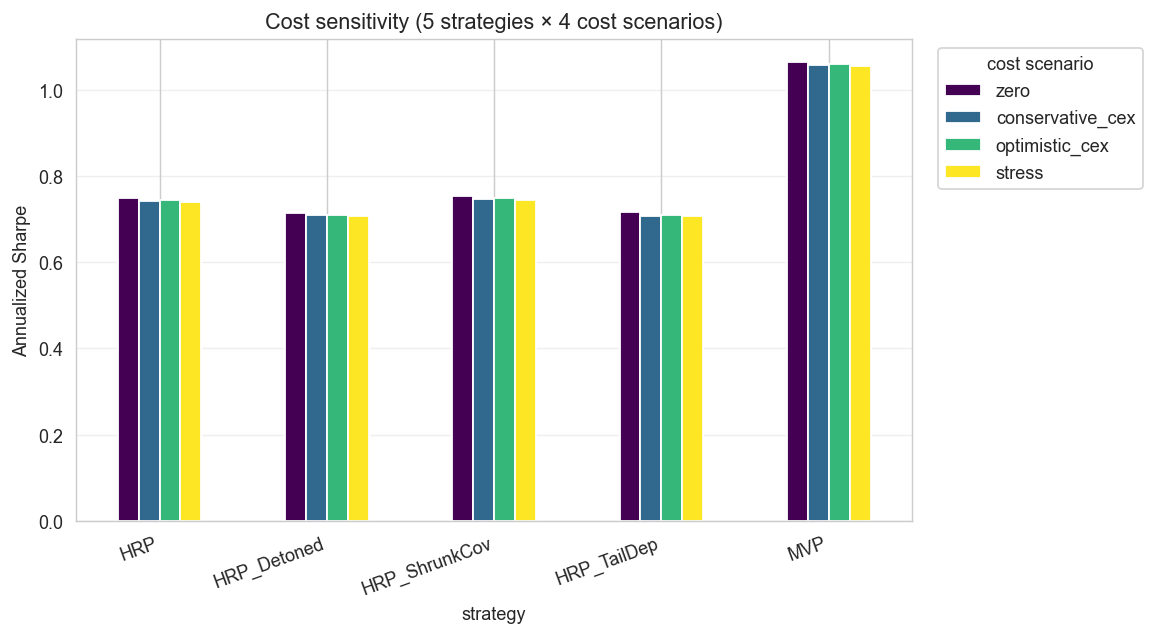
\includegraphics[width=0.85\textwidth]{figures/cost_sensitivity_sharpe.png}
  \caption{Cost-sensitivity grid. Rankings are robust across the four
  cost scenarios.}
  \label{fig:cost_sens}
\end{figure}

\begin{figure}[H]
  \centering
  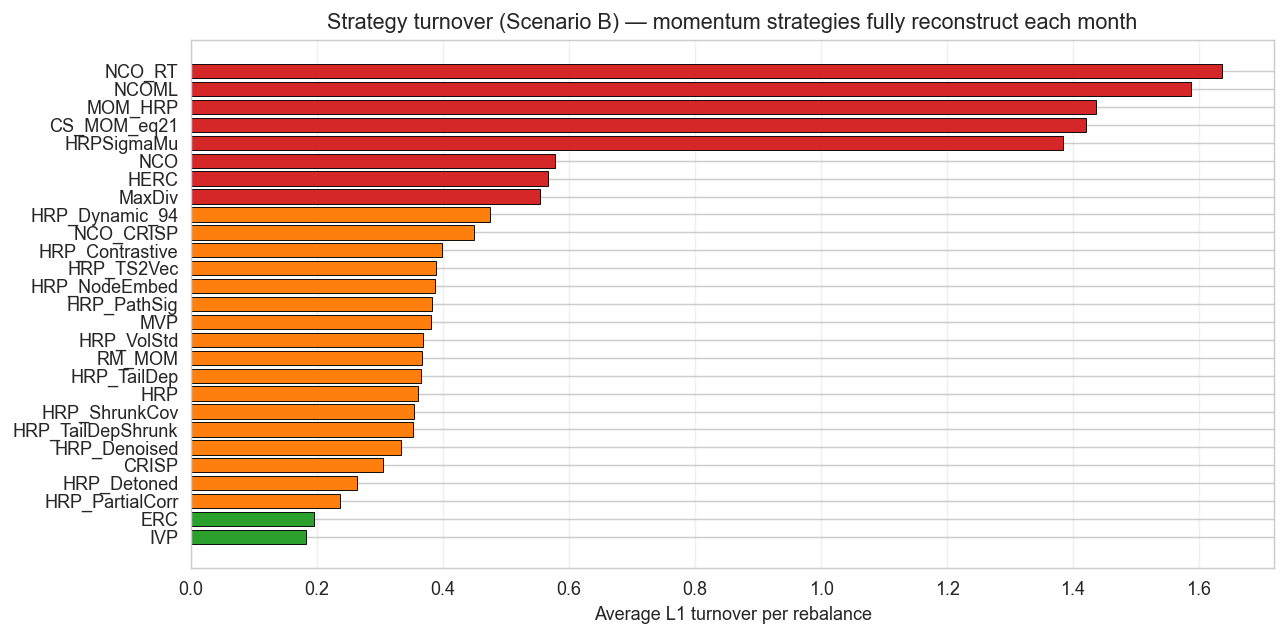
\includegraphics[width=0.95\textwidth]{figures/turnover_analysis.png}
  \caption{Average $L_1$ turnover per rebalance over time. Risk-based
  HRP variants and IVP cluster around $0.2$--$0.4$; momentum and the
  return-tilted strategies (CS\_MOM, MOM\_HRP, NCO\_RT, NCOML,
  HRPSigmaMu) carry $1.4$--$1.7$, an order of magnitude higher.
  Costs at the headline 10\,bps fee never alter the Sharpe ranking
  (Figure~\ref{fig:cost_sens}), but the gap shows where any
  liquidity-impact extension to the cost model would bite.}
  \label{fig:turnover}
\end{figure}

Threshold rebalancing (Scenario C, 5\% drift trigger) does not improve
on calendar rebalancing here: HRP's Sharpe edges down from $0.741$ to
$0.735$ and HRP\_ShrunkCov is essentially flat ($0.746 \to 0.745$),
with only a marginal turnover reduction. The smoothed variant
(Scenario C$'$) cuts turnover more materially, with HRP's average $L_1$
turnover falling from $0.36$ to $0.23$, at a modest Sharpe cost
($0.741 \to 0.731$). The momentum strategies are the exception:
RM\_MOM's volatility-targeting overlay needs to trade to function, and
suppressing or smoothing its rebalances collapses its Sharpe (from
$0.66$ under calendar rebalancing to $0.37$ under Scenario C and
$0.05$ under C$'$). Threshold logic suits low-turnover risk-based
strategies and actively harms turnover-dependent ones.

\subsection{Weekly cadence}
\label{sec:results-weekly}

The headline uses 76 monthly rebalances; crypto momentum is documented
to decay over 1--4 weeks \citep{liu2022cryptofactors}, so monthly
rebalancing may understate any faster-horizon edge. We re-ran the
non-embedding strategies at weekly cadence ($\sim$330 rebalances;
embeddings are excluded as retraining four encoders 330 times is
prohibitive). Two things change. First, \emph{every} strategy's Sharpe
rises (baseline HRP $0.74\to0.82$, NCO $0.93\to1.03$), and the momentum
family rises most (RM\_MOM $0.66\to0.92$, CS\_MOM $0.66\to0.91$),
consistent with momentum's short crypto half-life: monthly rebalancing
was simply too slow for it. Second, and despite the $\sim$4$\times$
larger rebalance count, the inference does \emph{not} sharpen: the
weekly Hansen SPA still gives $p_{\text{consistent}}=0.57$ (corrected
over the smaller, embedding-free weekly candidate set) and the
bootstrap Sharpe CIs stay $\sim$1.5 wide. More rebalances do not help
when the per-period return volatility is what dominates the standard
error. Higher cadence changes the \emph{ranking texture} (momentum
catches up) but not the \emph{statistical verdict}.

\subsection{Convergence findings (the structural results)}
\label{sec:results-convergence}

Two strategy pairs in our comparison are theoretically related: each
pair targets the same goal via different mathematical routes. We
quantify their weight-vector convergence across the full 76-snapshot
window (Figure~\ref{fig:detone_pc}).

\paragraph{HRP\_Detoned vs HRP\_PartialCorr.} Spectral detoning and
precision-matrix partial correlation both remove the dominant market
mode, by different routes. Across the 76 monthly snapshots their
weight-vector rank correlation is high but not invariant: mean Spearman
$\rho=0.87$, median $0.93$, with regime-driven dips to $\rho=0.54$ in
months when the dominant eigenvector shifts sharply. The bug-fixed
HRP\_PartialCorr ($\alpha=10^{-3}$) is now distinct from the
inverse-variance portfolio (its weight-rank correlation with IVP
averages only $\rho=0.08$), whereas the earlier degenerate
$\alpha=0.05$ implementation \emph{was} IVP. The detoning /
partial-correlation convergence is therefore a structural relationship
between two market-mode-removal estimators, not an artefact of one
collapsing into IVP.

\paragraph{HRP\_TailDep vs HRP\_TailDepShrunk.} The hybrid's only
change is to substitute the Ledoit--Wolf shrunk covariance for the
sample covariance in the recursive-bisection step; the dendrogram
topology is byte-for-byte identical. Spearman is 0.998--1.000 in
every snapshot tested. This is the most robust convergence finding
in our analysis: \emph{LW shrinkage in HRP's bisection step is a
within-cluster variance refinement that does not re-order the
dendrogram}.

\begin{figure}[H]
  \centering
  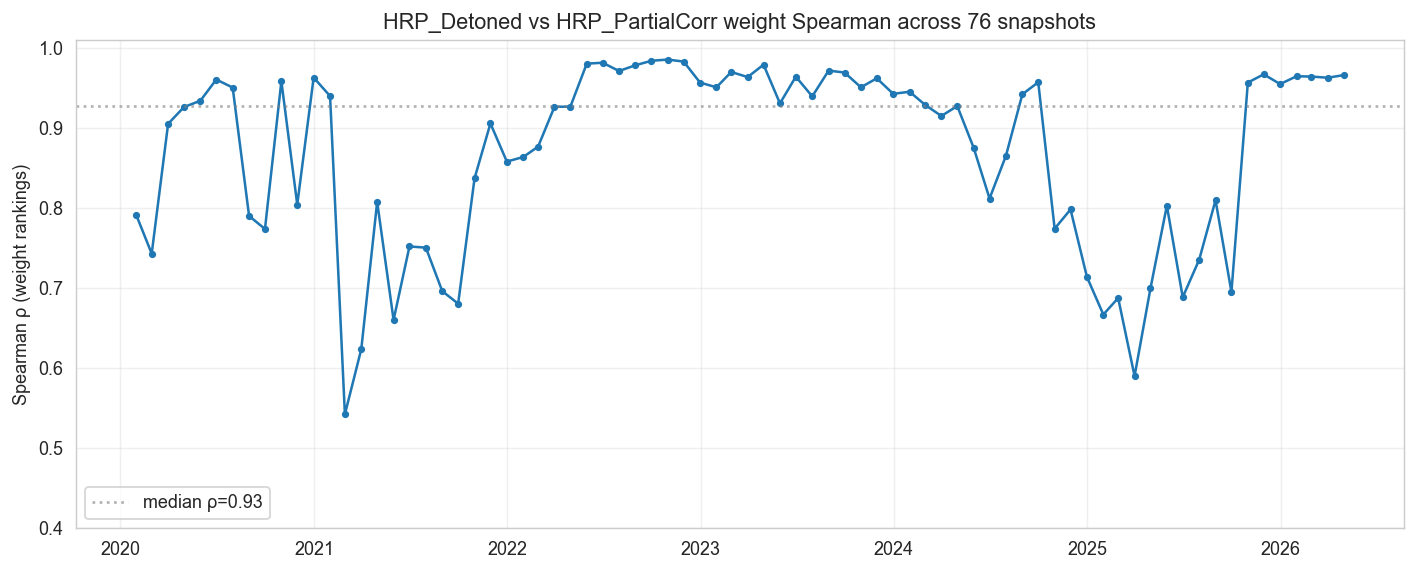
\includegraphics[width=0.95\textwidth]{figures/detoning_vs_partial_corr.png}
  \caption{Spearman rank correlation between HRP\_Detoned and
  HRP\_PartialCorr weight vectors across 76 monthly snapshots.}
  \label{fig:detone_pc}
\end{figure}

\subsection{Cluster stability: a retraction}
\label{sec:results-cluster}

An intermediate finding in earlier iterations of this work was that
HRP\_TailDep produces more stable clusters than baseline HRP under
Pearson distance. That claim was based on a \emph{single year-pair}
(2022-12-31 vs 2023-12-31) and showed Pearson ARI $=-0.047$ vs
TailDep ARI $=+0.265$ at $K=5$.

When we re-ran the analysis across all 76 monthly snapshots
(Figure~\ref{fig:cluster_stab}, Table~\ref{tab:cluster_stab}), the
direction reverses. \textbf{Pearson clusters are substantially more
stable than TailDep clusters at monthly resolution}: Pearson ARI
mean $+0.744$ vs TailDep $+0.614$; Pearson cophenetic mean $0.861$ vs
TailDep $0.768$. TailDep ARI exceeds Pearson ARI in only 23 of 75
month-pairs (31\%).

\begin{table}[H]
\centering\small
\caption{Cluster stability across 76 monthly snapshots (2020-2026).}
\label{tab:cluster_stab}
\begin{tabular}{lrr}
\toprule
Metric & Pearson distance & Lower-tail-dep distance\\
\midrule
Average cophenetic correlation & \textbf{0.861} & 0.768\\
Average ARI vs.\ previous snapshot (K=5) & \textbf{+0.744} & +0.614\\
Median ARI vs.\ previous snapshot & \textbf{+0.783} & +0.650\\
Months where TailDep ARI > Pearson ARI & --- & 23 / 75 (31\%)\\
\bottomrule
\end{tabular}
\end{table}

\begin{figure}[H]
  \centering
  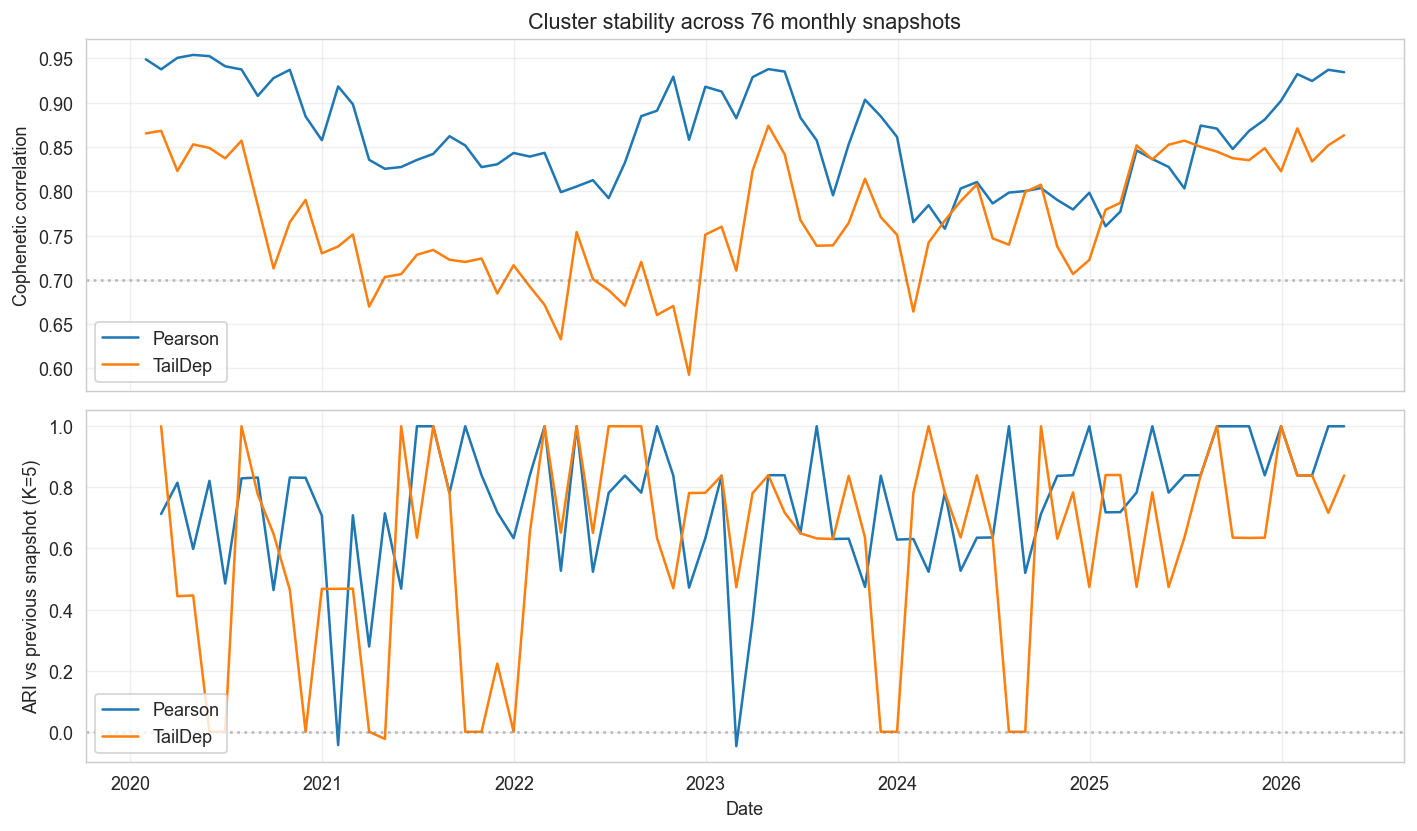
\includegraphics[width=0.95\textwidth]{figures/cluster_stability_timeseries.png}
  \caption{Cophenetic correlation (top) and ARI vs.\ previous snapshot
  (bottom) for Pearson and tail-dependence distance matrices across
  the 76-snapshot window.}
  \label{fig:cluster_stab}
\end{figure}

The economic argument for HRP\_TailDep, that it captures the
joint-crash co-movement structure Pearson summarises poorly,
\emph{stands}; the secondary cluster-stability argument \emph{does not}.
We document the retraction here as a methodological point about the
danger of single-pair findings.

%% ===========================================================================
\section{Discussion}
\label{sec:discussion}
%% ===========================================================================

The three threads of \S\ref{sec:results} converge on a single
argument. First, only one HRP design choice moves performance
materially: the allocation step. Across every clustering perturbation
we tried, no configuration escapes the HRP-family Sharpe band; the
strategies that do escape (NCO, CRISP, NCO\_CRISP, and the return-
tilted NCO that collapses) all change the within-cluster solve, and
the two signal-aware extensions (NCOML, HRP-$\Sigma\mu$) reinforce the
same message in opposite directions. Second, the strategies that do
move are too few to clear the multiple-testing correction: the Hansen
SPA and the Deflated Sharpe Ratio agree that no edge survives the
search, even where CRISP and NCO--CRISP clear the pairwise bar
comfortably. Third, the whole finding is regime-conditional: in the
post-COVID cut, diversified HRP variants lose half their capital
while concentration still wins, so much of what reads as
``diversification works'' in the full window is a residual on the
BTC rally. The practical conclusion sits at the intersection of the
three: HRP's signal-blindness is a feature in this market, the
allocation step is the main place where engineering effort appears to have paid
back, and even there the win is below what six years of data could
certify. The subsections below develop each thread in turn.

\subsection{Clustering versus allocation: the one design choice that
matters}
The results of \S\ref{sec:results} point to one practical conclusion.
Varying the \emph{clustering} step, across 547 hyperparameter cells,
did not separate a variant from baseline HRP; varying the
\emph{allocation} step did, in both directions (CRISP and the
NCO--CRISP hybrid to Sharpe $\approx0.98$, the return-tilted NCO to
$-97\%$). HRP and all its variants share one allocation rule,
inverse-variance recursive bisection, and that rule, not the
dendrogram, is what holds the family together. The NCO--CRISP hybrid
is the cleanest test: it places CRISP's correlation-shrinkage solve
inside NCO's hierarchical nesting, and lands \emph{between} its two
parents (NCO 0.93, CRISP 0.99): the shrinkage and the nesting are
substitutes, not complements. For a practitioner the implication is
narrow but useful: on this evidence, effort spent engineering the
clustering distance is lower-yield than effort spent on the allocation
objective.

The return-tilted NCO also speaks to a concurrent result.
\citet{wuebben2026crisp} reports, via Monte Carlo, that making a
hierarchical allocator return-aware improves out-of-sample Sharpe; our
live-market evidence is directionally different: a momentum-tilted NCO is
the worst strategy in the comparison. The two are reconcilable: a return
signal helps only when it carries genuine out-of-sample predictive
content, which a 63-day crypto-momentum signal over 2020--2026 does not.
Replacing the sample-mean tilt with a walk-forward XGBoost forecast
tests this directly. \textbf{NCOML}, the same nested-clustering
optimiser fed by the learned signal, reaches Sharpe $0.80$, sidestepping
the $-97\%$ collapse and suggesting the failure was mainly signal quality
rather than return-aware allocation in principle; but it also lands
\emph{below} pure (signal-blind) NCO at $0.93$, so the XGBoost forecast
is enough to avoid disaster but not strong enough to outperform NCO's
risk-only solve. \textbf{HRP-$\Sigma\mu$}, Wuebben's signal-aware
hierarchical optimiser fed by the same forecast, lands at $0.61$,
\emph{below} baseline HRP: in this sample, injecting a return signal into
HRP's hierarchy is associated with weaker performance, and the HRP family's strength is therefore in
its signal-blindness, not despite it. The simulation optimism and the
live-data behaviour together delimit when signal-aware hierarchical
allocation is worth attempting: a credible signal removes the collapse
but does not, on this universe and horizon, beat the signal-blind
allocators that already exist.

\subsection{Why does the Hansen SPA fail to reject, even for CRISP?}
CRISP and the NCO--CRISP hybrid each post a $\approx+0.24$ Sharpe edge
over HRP that is pairwise-significant (Ledoit--Wolf $p\approx0.01$) in
both the full and the post-COVID windows, yet the Hansen SPA
($p_{\text{consistent}}=0.51$) does not reject. This is not a
contradiction; it is the multiple-testing correction working as
intended. The pairwise test asks ``does \emph{this} strategy beat
HRP?''; the SPA asks ``does \emph{the best of 27 searched strategies}
beat HRP, given that we searched 27?'', and inflates the critical
value accordingly. CRISP's and NCO--CRISP's edges clear the first bar
and not the second. The honest reading is therefore specific: the two
shrinkage allocators show a real, regime-robust pairwise edge, but it
is not large enough to survive correction for the breadth of the
search: it is strongly suggested, not established.

\subsection{Regime conditionality}
Two regime-dependent findings frame the rest. Detoning and partial
correlation, both designed to remove the dominant market mode and
isolate idiosyncratic structure, underperform here because the dominant
mode \emph{was} BTC and being underweight BTC was costly; their value
is regime-dependent rather than a universal Sharpe improvement, and
the sideways or rotational regimes 2020--2026 did not contain may yet
reward them. The flip side is that a passive 100\% BTC hold (Sharpe
$0.87$, $+749\%$) beats every \emph{diversified} portfolio in the
comparison; the only constructed strategies above it, MVP and NCO, get
there by concentrating back into BTC, and that re-concentration is a
regime-conditional bet rather than a portfolio-construction insight.
The post-COVID cut is the counterweight: there, diversified HRP
variants lose 51--64\% while concentration still wins. Realised returns
over 2020--2026 have been dominated by the direction of BTC, and
inference about portfolio construction in this asset class has to be
conditioned on that fact.

\subsection{Limitations}
\begin{enumerate}
\item Statistical power. With six years of data the design cannot
    resolve a Sharpe edge below $\approx0.4$ for a strategy that
    departs substantively from HRP (\S\ref{sec:results-power}); NCO's
    economically large $+0.19$ edge is therefore left unresolved
    rather than confirmed or refuted.
\item Single venue (Binance USDT spot). A multi-exchange consolidated
    price (Kaiko, CCXT-aggregated) would give a more representative
    cost model but was out of scope for this paper.
\item No on-chain factors. The Liu-Tsyvinski-Wu \citep{liu2022cryptofactors}
    three-factor model and on-chain signals (Glassnode) are
    deferred to a follow-up.
\item PIT universe is ranked by Binance quote volume, not market cap.
    Pro-tier CoinGecko or paid Kaiko data would enable a market-cap
    robustness check.
\item Cross-platform reproducibility of trained-model strategies.
    Closed-form strategies are highly stable across environments, but
    strategies that rely on learned representations are only
    conditionally reproducible because platform-level floating-point
    differences can propagate through clustering and forecast-based
    allocation. In robustness checks, this affects the PyTorch-based
    embedding variants most, with Sharpe shifts on the order of
    $\approx 0.02$ and corresponding movement in marginal pairwise
    $p$-values. The main ranking structure and joint-test conclusions,
    however, remain unchanged.
\end{enumerate}

%% ===========================================================================
\section{Conclusion}
\label{sec:conclusion}
%% ===========================================================================

Across 27 constructed portfolio strategies tested against baseline HRP
on 76 monthly rebalances of a survivorship-bias-corrected Binance USDT
universe (2020--2026), the allocation step is the only HRP design
choice that materially moves performance, and even the strategies that
do move do not survive the multiple-testing correction. The roster
spans thirteen HRP-family variants (eight correlation/covariance
constructions and four embedding-based ones), five risk-based
comparators, four nested-clustering optimisers, three momentum
strategies and two signal-aware XGBoost-fed extensions; every
comparison is wrapped in a studentized Ledoit--Wolf test and the
reference Hansen SPA on a 146-ever-included-symbols point-in-time
universe.

Concretely: varying the \emph{clustering} step, that is the
correlation, distance, linkage or learned embedding that builds the
dendrogram, did not produce a detectable outperformance over baseline
HRP: across a 547-cell hyperparameter grid no configuration escapes
the HRP-family Sharpe band, and the combined Hansen SPA cannot reject
the null ($p_{\text{consistent}}=0.91$). The \emph{allocation} step
is more strongly associated with performance dispersion:
the CRISP correlation-shrinkage portfolio (Sharpe 0.99), an NCO--CRISP
hybrid (0.98) and NCO (0.93) all clear baseline HRP, while a
return-tilted NCO collapses to $-97\%$. Replacing that sample-mean
signal with a walk-forward XGBoost forecast sidesteps the collapse
(NCOML, Sharpe 0.80) without beating signal-blind NCO; feeding the
same forecast into Wuebben's signal-aware HRP-$\Sigma\mu$ underperforms
baseline HRP (0.61). CRISP and NCO--CRISP beat HRP at the pairwise
level in both the full and post-COVID windows (Ledoit--Wolf
$p\approx0.01$). But the Hansen SPA, correcting for the 27-candidate
search, still does not reject the null
($p_{\text{consistent}}=0.51$): no edge survives the multiple-testing
correction. The null is a statement about detectable, search-corrected
effect size rather than a proof of zero effect.

Two caveats frame the result. First, a passive 100\% BTC hold beats
every diversified portfolio, and the only constructed strategies that
beat \emph{it} (MVP, CRISP, NCO--CRISP, NCO) win by concentrating back
into BTC; in this asset class and regime, portfolio construction has
been second-order to the BTC beta. Second, in the post-COVID sub-sample
every diversified HRP variant lost 51--64\% of capital, so the
``diversification works'' reading of the full window is itself
regime-conditional. We also retract an earlier cluster-stability claim
that the 76-snapshot re-analysis falsifies.

The paper's contribution is an empirically-tested map of which HRP
design choices affect performance: of the many parameters an HRP
practitioner can vary, the allocation objective is the component most
consistently associated with
detectable change, and even the strategies that improve on baseline
(CRISP, NCO--CRISP) do so by an edge that does not survive correction
for the number of strategies tried.

Several directions remain open for future work. Time-varying
conditional covariance (DCC-GARCH) would give the dynamic-correlation
layer a properly
conditional second moment in place of the EWMA recursion.
Regime-switching analysis could test directly whether detoning and
partial correlation, which underperform in the BTC-led 2020--2026
window, add value in the sideways or rotational regimes that window
did not contain. On-chain factors \citep{liu2022cryptofactors} and a
multi-exchange consolidated price (e.g.\ Kaiko) for a venue-robust cost
model are natural data extensions. The most concrete empirical
follow-up, though, is a longer out-of-sample window: the power analysis
(\S\ref{sec:results-power}) shows NCO's $+0.19$ Sharpe edge cannot be
certified on six years of crypto data, and the post-COVID cut suggests
that at least one embedding variant can edge \emph{ahead} of baseline
HRP in choppier regimes while the others remain close. This signal is too weak to confirm here but
worth revisiting once more non-bull data accrues. The NCO result also
invites a closer study of \emph{why} a nested minimum-variance
allocation tends to separate from the HRP pack in this sample.

\section*{Acknowledgements}

We thank the UCEMA
Quantitative Finance faculty, particularly Manuel Maurette and Pablo
Martin Gechidjian, for their support and feedback. Finally, we thank
Marcos L\'opez de Prado for developing the foundational Hierarchical
Risk Parity framework that this study extends.

\bibliographystyle{plainnat}
\bibliography{references}

\end{document}
